% Template for a Computer Science Tripos Part II project dissertation
\documentclass[12pt,a4paper,twoside,openright]{report}
\usepackage[pdfborder={0 0 0}]{hyperref}    % turns references into hyperlinks
\usepackage[margin=25mm]{geometry}  % adjusts page layout
\usepackage{graphicx}  % allows inclusion of PDF, PNG and JPG images
\usepackage{verbatim}
\usepackage{amssymb}
\usepackage{amsmath}
\usepackage{docmute}   % only needed to allow inclusion of proposal.tex
\usepackage{listings}  % for formatting code
\usepackage{longtable}
\usepackage{csvsimple}
\usepackage{float}
\usepackage[linesnumbered,figure,vlined]{algorithm2e}
\floatstyle{boxed} 
\restylefloat{figure}

\raggedbottom                           % try to avoid widows and orphans
\sloppy
\clubpenalty1000%
\widowpenalty1000%

\renewcommand{\baselinestretch}{1.1}    % adjust line spacing to make
                                        % more readable

\lstset{
  basicstyle = \footnotesize\ttfamily,
  columns = fullflexible,
  keepspaces = true,
  keywordstyle = \bf
}

\begin{document}
\SetKwProg{Fn}{Function}{:}{end}

\bibliographystyle{plain}


%%%%%%%%%%%%%%%%%%%%%%%%%%%%%%%%%%%%%%%%%%%%%%%%%%%%%%%%%%%%%%%%%%%%%%%%
% Title


\pagestyle{empty}

\rightline{\LARGE \textbf{Lauren Pick}}

\vspace*{60mm}
\begin{center}
\Huge
\textbf{A Model Checker Using IC3} \\[5mm]
Computer Science Tripos -- Part II \\[5mm]
Homerton College \\[5mm]
\today  % today's date
\end{center}

%%%%%%%%%%%%%%%%%%%%%%%%%%%%%%%%%%%%%%%%%%%%%%%%%%%%%%%%%%%%%%%%%%%%%%%%%%%%%%
% Proforma, table of contents and list of figures

\pagestyle{plain}

\chapter*{Proforma}

{\large
\begin{tabular}{ll}
Name:                  & \bf Lauren Pick                           \\
College:               & \bf Homerton College                      \\
Project Title:         & \bf A Model Checker Using IC3             \\
Examination:        & \bf Computer Science Tripos -- Part II, 2016 \\
Word Count:            & \bf                                       \\
Project Originator:    & Lauren Pick                               \\
Supervisors:           & Dr Dominic Mulligan, Dr Ali Sezgin        \\ 
Supporting Supervisor: & Prof Alan Mycroft
\end{tabular}
}


\section*{Original Aims of the Project}

Describe the original aims of the project, i.e. summarize information from
the ``Substance and Structure'' and ``Success Criteria'' sections of the
project proposal.

\section*{Work Completed}

Describe the work completed as part of project, including extensions.

\section*{Special Difficulties}

None.
 
\newpage
\section*{Declaration}

I, Lauren Pick of Homerton College, being a candidate for Part II of the Computer
Science Tripos, hereby declare
that this dissertation and the work described in it are my own work,
unaided except as may be specified below, and that the dissertation
does not contain material that has already been used to any substantial
extent for a comparable purpose.

\bigskip
\leftline{Signed [signature]}

\medskip
\leftline{Date [date]}

\tableofcontents

%\listoffigures

%\newpage
%\section*{Acknowledgements}


%%%%%%%%%%%%%%%%%%%%%%%%%%%%%%%%%%%%%%%%%%%%%%%%%%%%%%%%%%%%%%%%%%%%%%%
% now for the chapters

\pagestyle{headings}

\chapter{Introduction}

This project focuses on implementing the IC3 algorithm, a SAT-based model checker. 
To provide context for the project,
I provide a brief introduction to formal verification and model checking, followed
by a discussion of symbolic model checking and SAT-based model checking.
I then highlight some of the important features of the IC3 algorithm and its more
recent uses.

%Provide a brief description of model checking in general.

Formal verification is the use of mathematics and logic to prove properties of
hardware and software systems. Formal verification techniques are
employed in several domains where the correctness of a system is
crucial, such as in hardware design and aviation.
Guaranteeing that there are no errors in hardware designs before
manufacturing begins can help avoid the high costs associated with needing to
remanufacture the hardware if the design needs to be corrected.
Additionally, the ability to prove that certain kinds of errors do not
occur are important for ensuring safety in safety-critical systems such
as those in airplanes and medical devices.

One formal verification technique is model checking.
Given a model of the system
and a specified property, a model checker will check
whether all reachable states in the system satisfy this property.
Unlike formal verification techniques that employ Hoare Logic
and theorem provers that require user guidance, model checking
is a fully automated verification technique.

In addition to being automated, because model checkers prove
properties by considering reachable states, when a model checker
discovers that a property does not hold, the model checker has
necessarily discovered a reachable state that violates the property.
A counterexample trace can, in such cases, be provided, giving
greater insight into why the property does not hold for that
model.


\section{Symbolic Model Checking}

%Discuss BDD-based and SAT-based model checking techniques.
All model-checking approaches suffer from limitations on the size
of the systems they can model check in practice as a result of
the state explosion problem: the number of
states in a system can be (and often is) exponential in the
number of state variables \cite{clarke12}. 

The initial approach to the model checking problem involved explicitly
considering each reachable state in the model.
Symbolic model checking arose as a method of mitigating the effects of
the state explosion problem to some extent. By representing
states and the transition relation between them as boolean
expression, symbolic model checking allows sets of states to be
represented efficiently as boolean expressions involving state variables
as opposed to an explicit list of each individual state in the set
\cite{mcmillan92}. 

Symbolic model checking was originally invented for use with ordered
binary decision diagrams (BDDs), data structures that provide an efficient
representation of propositional formulas. A unique BDD represents each logical
formula given a particular variable ordering, and an implementation that
only stores each BDD once and uses pointers appropriately can result in
less space being used.
The efficiency of BDDs in storing propositional formulas allowed for the model
checking of systems with larger numbers of states than could be handled
by explicit-state model checking \cite{mcmillan92}.

% Transition into talking about SAT-based model checking
The efficiency of BDD representations relies on choosing an appropriate
ordering, which can be computationally expensive, and in some cases,
there is no such ordering that results in a space-efficient BDD
\cite{biere99a}.

An alternative to BDD-based symbolic model-checking techniques are SAT-based
techniques, which do not use the canonical representations of propositional
formulas as BDDs and make use of procedures for solving the boolean
satisfiability problem.
Such techniques include bounded model checking (BMC),
which proves properties by finding counterexamples of certain lengths
\cite{biere99a};
$k$-induction, which proves properties inductively \cite{sheeran00};
and the IC3 algorithm that is the focus of this project.
% Mention FSIS?
% Mention ITP?

Many modern SAT-based model checkers are based on BMC, which begins at the
initial state of the transition system and searches for paths of length
$k$ from the initial state that violate the negated property.
If no path of length $k$ is found, BMC increments $k$ and searches again.
BMC is effective at finding counterexamples, but for some large systems,
BMC is incomplete unless it is allowed to reach the point at which $k$ is
the maximal path length.

The $k$-induction algorithm is similar to BMC in its unrolling of the
transition relation to consider paths of length $k$, but it also
incorporates induction. At each depth $k$, the algorithm asserts that the
desired property holds at each state before the final state.

% Understanding IC3

\section{The IC3 Algorithm}

%Give context for the IC3/PDR algorithm, e.g. history and comparisons
%with other SAT-based model checking algorithms such as BMC and $k$-induction.

The IC3 algorithm (also called PDR \cite{een11}) is a SAT-based model-checking
algorithm for proving the safety properties (i.e. properties that must hold
in all reachable states) of hardware.
The first implementation of the algorithm \verb,ic3, placed third in
the 2010 Hardware Model Checking Competition (HWMCC'10), a competitive event
that receives model checker and benchmark submissions from industry and
academia. Its performance at HWMCC'10 generated interest in the algorithm, and
since then, several variants of the algorithm have been developed.
%2015 paper

As in $k$-induction, properties are proved through induction:
the algorithm considers reachable sets of states $k$ steps away from the
initial state until reaching a fixed point.
% Note: find when k-induction started using counterexamples
As with later variants of $k$-induction, the IC3 algorithm also discovers
new invariants if the initial assumptions are not strong enough to prove
the desired property, but unlike $k$-induction, the safety property guides
the discovery of the invariants. As a result, the discovered invariants
are more relevant for proving the safety property \cite{bradley12}.

Furthermore, IC3 does not unroll the transition relation as $k$-induction
or other BMC-based methods do, but instead considers at most one step
of the transition relation at a time, leading to smaller,
simpler SAT queries. As a result, IC3 requires less memory than BMC-based
methods in practice \cite{bradley12}.


\section{Further Work}

%Mention other applications of the IC3 algorithm, e.g. to checking
%LTL properties and to software model checking.

%Mention IIV?

While IC3 algorithm is for model checking safety properties of hardware,
there are applications of the algorithm in model checking LTL and CTL
properties and model checking software \cite{bradley12}.

The FAIR model-checking algorithm, which model checks $\omega$-regular
properties, makes use of a safety model checker such as IC3, and IICTL,
which model-checks CTL formulas \cite{hassan12}, makes use of both a
safety model checker such as IC3 as well as a fair cycle finder such as
FAIR.

Other work generalizes IC3 to use an underlying SMT solver rather than a
SAT solver, and this generalization has been used to check control-flow
graphs of programs \cite{cimatti12}.
More recently, Johannes Birgmeier, Aaron Bradley, and Georg Weissenbacher
have introduced CTIGAR, a method of abstraction-refinement based on IC3's
counterexamples to induction rather than the counterexamples in CEGAR,
which experiments suggest is competitive with CEGAR-based techniques for
software verification \cite{birgmeier14}.

\section{Project Aims}

This project's main aim is to implement a basic form of the IC3 algorithm in
Haskell that should be able to correctly check several
small examples. Additionally, the project is meant to give me an opportunity
to learn and use Haskell, to understand formal methods and especially model
checking more deeply, and to put into practice software engineering techniques.

I have successfully implemented not only a basic form of the IC3 algorithm,
which can correctly check several examples from the hardware model checking
competition in addition to the small hardware models I initially set out
to check, but also several variants of the algorithm.

\chapter{Preparation}

This chapter describes the knowledge gained and plans made while preparing
to being writing code for the project.
The preparation for the project involved learning Haskell, distinguishing
the main components of the project, choosing and learning how to use
the necessary tools for implementing the components of the project,
and gaining the necessary knowledge about the IC3 algorithm.

\section{Haskell}

The majority of the code for the project is implemented in the functional
programming language Haskell. I explain some features of the
language that should help with understanding future code snippets
by comparison with Standard ML.

%Type signature syntax
\paragraph{Types}{
Similarly to Standard ML, Haskell compilers perform type inference, but type
signatures can be (and, in some cases where type inference cannot resolve
ambiguities, must be) provided. For example, the type signature for the
\verb,prove, function in the model checker, a curried function
that takes a \verb,Model, and a \verb,Lit, and returns a \verb,Bool,,
implementation is given in figure \ref{typesigexample}.

\begin{figure}[!ht]
\begin{lstlisting}
prove :: Model -> Lit -> Bool
\end{lstlisting}
\caption{The type signature for the {\tt prove} function.}
\label{typesigexample}
\end{figure}

%Type constructors
Haskell type constructors work similarly to Standard ML type constructors,
with the main difference being that Standard ML's \verb,datatype, is instead
\verb,data, in Haskell.

Haskell also provides record syntax for creating new types, allowing components
to be named.
}

%List syntax
\paragraph{Lists}{
The model checker implemented as part of this project makes extensive use
of lists. List types in Haskell are denoted using square brackets, i.e.
a list of \verb,Lit,s has type \verb,[Lit],.
Lists can be appended using the \verb,++, infix operator, and elements
can be prepended to lists using the infix operator \verb,:,. For
example, the Haskell equivalent to the Standard ML expression \verb.1::[2,3,4] @ [5,6].
is \verb.1:[2,3,4] ++ [5,6]..}

%Modules
\paragraph{Modules}{
A Haskell program consists of modules, which are used to organize code.
Modules (or just selected functions from modules) can be imported into other
modules, which is how library functions can be used.
}

\section{Requirements Analysis}

%Describe the requirements for the project: AIGER parser, Minisat interface,
%transition system representation, algorithm implementation.

The model checker requires a way of taking input models and also
requires a way to solve SAT queries.
I chose the AIGER format for representing the hardware models and the
MiniSat SAT solver for answering SAT queries, resulting in a need for an
AIGER parser and a Haskell interface to MiniSat. The choice of
the AIGER format allows the model checker to be run on examples from
the Hardware Model Checking Competition (HWMCC), since this is the format used
to specify examples in the competitions. I chose the MiniSat SAT
solver because it is the SAT solver used by Aaron Bradley's reference
implementation of IC3 that this implementation is to be compared against.

Given that the model checking algorithm deals with transition systems
(discussed later), the implementation also requires a representation of
transition systems, which should correspond to the input hardware model.
A further requirement is the implementation of the
IC3 algorithm itself.

The main required components are thus the AIGER parser, MiniSat interface,
transition system representation, and IC3 algorithm implementation.

\section{Tools Used}

I used a variety of tools to employ software engineering practices, such
as version control and testing, and to otherwise ease the development of
the project's code.

\paragraph{Git}{
The Git version control system was used for managing the project's code. The
previous versions maintained by the version control system proved useful in
the development of the code, and branching and merging capabilities were
useful for working on and organizing different variations of the model checker.
Git submodules, which allow the inclusion of other Git projects within another
project, were used to include MiniSat within the project, enabling easier
acquisition of project dependencies (i.e., MiniSat can be obtained by running
\verb,git submodule init, after running \verb,git clone, to clone the repository).

GitHub, a widely-used hosting service for Git repositories, was used to keep
backups of the code.}

\paragraph{Haddock}{
The Haddock documentation tool for Haskell was used to generate documentation
for the code. Haddock automatically generates documentation in
several formats (e.g. HTML) from annotated Haskell code. It is commonly
used to document Haskell code, being used for most packages available
on Hackage.
}

\paragraph{HUnit}{
HUnit is a framework for writing unit tests in Haskell based on the JUnit framework
for unit testing in Java. HUnit allows tests to be specified by using functions
that return the \verb,Assertion, type to write \verb,TestCase,s. For example, the
\verb,assertBool :: String -> Bool -> Assertion, function takes a \verb,String,
that gives an error message and a \verb,Bool, value, and raises an exception (with
the error message) if the \verb,Bool, is not \verb,True,, so the following
expression would give a \verb,TestCase, that tests that function
\verb,isEven, returns \verb,True, when called with parameter 12:
\begin{verbatim}
TestCase (assertBool "Error: (isEven 12) results in False" (isEven 12))
\end{verbatim}
\begin{figure}[h]
\centering
\begin{lstlisting}
data Test = TestCase Assertion
          | TestList [Test]
          | TestLabel String Test
\end{lstlisting}
\caption{The HUnit {\tt Test} datatype}
\end{figure}

The \verb,Test, datatype in HUnit allows \verb,Test,s to be grouped
and built up hierarchically. Tests that have been assembled into a
singly tree can then be treated as a test suite, and the whole tree
of unit tests can be run.}

\paragraph{Criterion}{
Criterion is a library for performing benchmarking in Haskell.
Criterion can output benchmarking results in any format specified in the \verb,.tpl,
template format, and by default outputs to HTML.
The \verb,.tpl, file can be configured such that
Criterion can, for example, output benchmark sample results to a CSV, as the
\verb,.tpl, for benchmarking this project was configured.}

\paragraph{Cabal}{
Cabal is the standard package and dependency management system for Haskell,
where a package may be either a library or a complete piece of software.
A \verb,.cabal, file in the root directory of a project specifies
information about a Cabal package, such as its version and dependencies,
The \verb,.cabal, file may contain several different sections, such as a
\verb,library, section, describing the modules in the package that should be
exposed in the library provided by the package or an \verb,executable, section,
which has fields for specifying the Haskell file containing the \verb,Main,
module and for specifying other Haskell files used by the program.
The \verb,.cabal, file for this project also uses the \verb,Test-Suite, section
to allow the HUnit test for the project to be run in a standard way (by running
\verb,cabal test, in the root directory of the package) and the \verb,Benchmark,
section to allow the benchmarking program to be run in a standard way as well
(by running \verb,cabal bench, in the root directory of the package).

Cabal also uses a Haskell file \verb,Setup.hs, to give further information
about how to build the package. For example, the \verb,Setup.hs, file
for this project compiles the C and C++ code needed for the project before
Cabal attempts to build the rest of the project, so the files necessary
for linking are already present.

The use of Cabal enables the project to be built easily on different platforms,
since Cabal provides a standard method for building the package that works
across platforms.}

\paragraph{hsc2hs}{
The \verb,hsc2hs, preprocessor eases the writing of Haskell bindings to C
code by enabling the programmer to write a \verb,.hsc, file containing
macros that the preprocessor can expand to, e.g., pointer offsets. The
\verb,hsc2hs, expands the macros in a \verb,.hsc, file to produce a
\verb,.hs, file that can then be compiled with a Haskell compiler and run.
}

\paragraph{HLint}{
The HLint tool suggests improvements for Haskell source code to improve
the style of the code. The incorporation of HLint suggestions in
the project resulted in simpler, more readable code.
}

\paragraph{Aiger Utilities}{
Several tools provided in Aiger Utilities were used in the project. The
AIGER parser provided was used for comparison with and as an alternative
to the one developed as part of this project. 

The Aiger Utilities' tools to convert between formats for specifying
hardware models eased the specification of new hardware models that would
be compatible with the model checker, which accepts only AIGER-formatted inputs.
In particular, the tools of use were
the {\tt bliftoaig}
tool, which converts a circuit specified using the Berkeley Logic Interchange Format
to a circuit specified using the binary AIGER format, and the {\tt aigtoaig} tool,
which converts between the ASCII and binary AIGER formats.
}

\paragraph{MiniSat}{
MiniSat is a SAT solver implemented in C++ that solves boolean satisfiability problems
posed in conjunctive normal form. Further details are given in section \ref{MiniSat}.
}

\section{Symbolic Representation}
\label{logic}

Symbolic model checkers rely on the representation of the underlying system as a
transition system, which describes the behavior of the system as one-step transitions
between states. Transition systems and states are themselves defined using
propositional logic formulas.

I give a brief review of concepts in logic before formally defining transition systems
and explaining how propositional logic formulas represent states.

\paragraph{Logic}{
Unless otherwise specified, a variable is a propositional symbol,
and can be assigned to boolean values {\it True} or {\it False}.
A \emph{literal} is defined as being either a variable $v$ or its negation $\neg v$.

The concepts of a cube and a clause are useful in describing the
representation of states as logical formulas.
A \emph{cube} is defined to be a conjunction of literals and may be represented as the set
of literals that occur in it. Similarly, a \emph{clause} is a disjunction of literals that
may also be represented as the set of literals that occur in it.

Given a cube $c$, a $d$ is a \emph{subcube} of $c$ (written $d \subset c$)
iff the set of literals in $d$ are a subset of the set of literals in $c$.
Similarly, given a clause $c$, a clause $d$ is a \emph{subclause} of $c$ (also
denoted $d \subset c$) iff the set of literals in $d$ are a subset of
the literals in $c$.

Through the application of deMorgan's laws, the negation of a cube is a clause and
vice-versa. In particular, a cube $C = l_0 \wedge \ldots \wedge l_n$ has negation
$\neg C = \neg (l_0 \wedge \ldots \wedge l_n)$, which is logically equivalent,
by deMorgan's laws, to the formula $\neg l_0 \vee \ldots \vee \neg l_n$.
Similarly, a clause $D = l_0 \vee \ldots \vee l_n$ has a negation that is
logically equivalent to $\neg l_0 \wedge \ldots \wedge \neg l_n$. It follows
that the clause obtained by negating a cube is specified by the set obtained
by negating each literal in the cube set and that the cube obtained by negating
a clause is specified by the set obtained by negating each literal in the clause.

A propositional formula is in \emph{conjunctive normal form} (CNF) iff it is a conjunction 
$\bigwedge_i D_i$ of disjunctions $D_i$ of literals (i.e. clauses). A set of clauses
can be interpreted as the CNF formula resulting from the conjunction
of the clauses.}

\paragraph{Transition Systems}{
A \emph{transition system} is a tuple $(i,x,I,T)$ consisting of a set of input
variables $i$, state variables $x$, an initial
set of states represented by the logical formula $I(x)$ and
a transition relation represented by the logical formula $T(i,x,x')$,
where $x'$ is the set of next-state variables.

For each state variable $v$, $v'$ denotes the corresponding next-state variable.
For example, a transition relation that states that all variables that are
currently {\it True} should become {\it False} in the next state is as follows:
$$T(i,x,x') = \bigwedge_{v \in x} (v \Rightarrow \neg v').$$

Given transition relation $(i,x,I,T)$, a logical formula $C$ is, by definition,
\emph{inductive relative} to another logical formula $F$ if both
$I \Rightarrow C$ and $F \wedge C \wedge T \Rightarrow C'$ hold.
}

\paragraph{States}{
A single state of the transition system (or a singleton set containing that state)
is specified through the assignment of all variables in the transition system
to boolean values, where a \emph{complete} assignment is represented as a cube such
that every variable appears in the formula exactly once.
An incomplete assignment of variables in the transition system is a cube such that
at least one variable in the transition system does not appear in the cube. Such an
assignment $c$ specifies the set of cubes $\{a \in{\it Full~Assignment}|c \subset a\}$,
where ${\it Full Assignment}$ is the set of complete assignments to the variables in the
transition system.
More generally, any logical formula $b$ involving the variables in the transition
system gives the set of states
$\{a \in {\it Full~Assignment} | a \wedge b~{\rm is~satisfiable}\}$.

A state that is in the set of states represented by a logical formula $B$ is referred to
as a $B$ state. A set of states $s$ is said to be reachable
in $k$ steps of the transition relation iff there exist states $s_0, \ldots, s_k$ such that
$s_0$ is an $I$ state and $s_i \wedge T \Rightarrow s_{i + 1}$ for $1 \leq i < k$.

}


\section{Model Specification}
%Describe the AIGER (old and new version) and BLIF formats and
%{\tt bliftoaig} from the AIGER utilities.

%Comments?

I used both the AIGER format and Berkeley Logic Interchange Format (BLIF)
to specify fourteen example hardware models.
The hardware models that the model checker accepts as input
are specified using the AIGER format;
however using the AIGER format to specify larger models was cumbersome,
so such models were specified using BLIF and converted to AIGER format
using the Aiger Utilities' \verb,bliftoaig, tool.

Inputs to model checker are models formatted using either the ASCII or
binary versions of the AIGER format.
The AIGER format provides a method of specifying hardware modeled as
And-Inverter Graphs with latch elements providing single clock-tick
delays: all circuits are modeled as a graph of nodes consisting only of
AND gates, inverters, and latches, where the latches behave like D
flip-flops, outputting the value of the current input at the next
clock tick.

The AIGER format has both an ASCII and a binary version. The ASCII
format is more flexible and human readable, imposing fewer constraints
on the ordering of components within the input file. For example, an
AND gate with variable name 20 may be specified before an AND gate with
variable name 11 in the ASCII format, but AND gates must be specified in
ascending order of their variable names in the binary AIGER format. Another
example is that AND gates' inputs can be specified in any order in the ASCII
format, but the binary format encodes AND gates under the assumption
that inputs are specified in ascending order.
The the binary version's assumptions on component ordering allows the format
to be more compact. The HWMCC examples use the binary format.

A new version of the AIGER format is currently under development, with
examples from HWMCC'14 using the new version. The AIGER parser implemented
as part of this project handles both the old and new versions of the AIGER
format.

\paragraph{AIGER Variables}{
A variable's name in AIGER format is a positive integer. Variables themselves
are not represented directly in AIGER format; instead, nonnegative numbers
are used to represent literals.
I will refer to these nonnegative numbers as indices.

For any variable named $x$, the index for positive literal $x$ is given by
$2 \times x$, and the index for negative literals $\neg x$ is given by
$2 \times x + 1$, i.e. a function to map from variable names $x$ and a boolean
value $b$ giving the sign of the literal would be as follows:
$${\it index}(x, b) =
\begin{cases}
2x & {\rm if}~b \\
2x + 1 & {\rm otherwise}
\end{cases}$$
The indices 0 and 1 are used to represent the constant boolean values {\it False}
and {\it True}, respectively.

Any index above 1 represents a literal and that for all such
indices, all even indices represent positive literals, and all odd indices
represent negative literals. The representation thus allows an implementation
use the least significant bit of an index to be used to find the sign of a literal,
and a single bitwise right shift to find the variable name for the literal.

\paragraph{Old version}{
All AIGER files in the old version begin with a header of the form
\begin{verbatim}
V M I L O A
\end{verbatim}
where
\begin{itemize}
\item \verb,V, can take on values \verb,aag,, specifying that the file is in the ASCII format or \verb,aig,,
specifying that the file is in the binary format.
\item \verb,M, gives the maximum index of a variable.
\item \verb,L, gives the number of latches.
\item \verb,O, gives the number of outputs.
\item \verb,A, gives the number of two-input AND gates.
\end{itemize}

The different components are specified after the header
in the order that their counts are given in the header.

In the ASCII version of the format, inputs are specified by giving the
index that represents the positive literal for its corresponding variable name,
and outputs are specified similarly as single indices (that may represent
literals of any sign).

Latches have initial value 0 (i.e., {\it False}) and are specified by giving the
index representing the positive literals for their corresponding variable name
followed by the index for their next-state value.
AND gates are specified by giving the indices that represent the positive literal
for their variable name and the two indices that specify their input values.

\begin{figure}[h]
\centering
\begin{verbatim}
aag 3 0 2 1 1
2 3
4 2
6
6 2 4
\end{verbatim}
\caption{
A circuit specified in the old ASCII AIGER format
}
\label{aagCircuit}
\end{figure}

\begin{figure}[h]
\centering
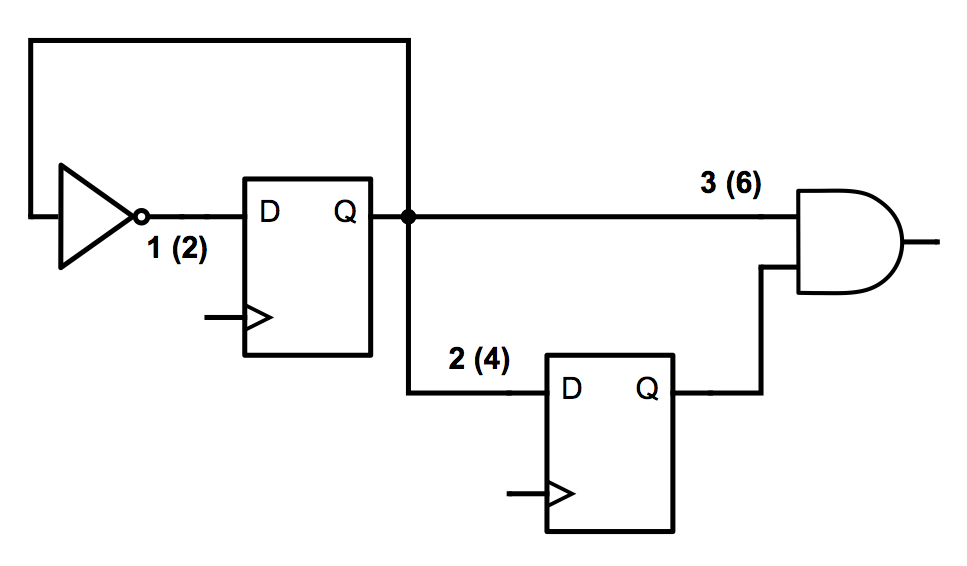
\includegraphics[width=100mm]{circuit.png}
\caption{The circuit represented by figure \ref{aagCircuit}, where
the variable name for each component is directly to the left of that
component, with the corresponding index in parenthesis.}
\end{figure}

For example, figure \ref{aagCircuit} specifies a circuit with
no inputs, two latches with indices $2$ and $4$ and one AND gate
$6$ that takes the outputs of the two latches as inputs and whose
output is the single output of the circuit.}

\paragraph{Binary version}{
The binary version of the format assumes that variable indices
occur in increasing order. Since each literal must be defined, this assumption
allows for variable indices to be omitted when defining inputs or latches.

Inputs are not explicitly listed; the input variables are inferred based on
the value of \verb,I,.
Similarly, latches are specified by only listing their next-state literals'
representations.

The binary format also assumes that AND gates occur in order of their
variable indices and that inputs to an AND gate will
have already been defined before that AND gate.
These assumptions allow AND gates to be represented by two differences
that tend to be small in practice:

For an AND gate specified in the old format by \verb,lhs rhs0 rhs1,,
where inputs \verb,rhs0, and \verb,rhs1, have been ordered such that
$\verb,rhs0, \geq \verb,rhs1,$, define
$$\delta_0 = \verb,lhs, - \verb,rhs0,$$
and
$$\delta_1 = \verb,lhs, - \verb,rhs1,$$

The values $\delta_i$ are then represented with the following binary
encoding, giving a more compact representation for AND gates than
the ASCII version of the format:

For 7-bit words $w_0, \ldots w_n$ with
$$\delta_i = w_0 + 2^7w_1 + \ldots + 2^{7n}w_n,$$
$\delta_i$ is represented as the sequence of $n + 1$ bytes
$b_0, \ldots, b_n$, where
\begin{itemize}
\item for $0 \leq k < n$, $b_k$ is the byte obtained by setting the most
significant bit to 1 and the rest of the bits to $w_k$, and
\item $b_n$ is the byte obtained by setting the most
significant bit to 0 and the rest of the bits to $w_n$
\end{itemize}}


\paragraph{New version} {
The new AIGER format begins with a header of the form
\begin{verbatim}
V M I L O A B C J F
\end{verbatim}
where \verb,V,, \verb,M,, \verb,I,, \verb,L,, \verb,O,, \verb,A, are as
in the old format, and
\begin{itemize}
\item \verb,B, gives the number of ``bad state'' properties
\item \verb,C, gives the number of invariant constraints
\item \verb,J, gives the number of justice properties
\item \verb,F, gives the number of fairness constraints
\end{itemize}

The ``bad state'' properties allow for the specification of properties for
a model checker to prove are unreachable separately from the outputs; in
the old AIGER format, such properties had to be specified as outputs.
The invariant constraints allow for the specification of properties that
are true at all states up to and including the state where the ``bad state''
is found.
Justice and fairness constraints are not included in the model used by
the model checker and will not be explained further.

Components are specified after the header in the same order that their
counts are given in the header with the exception of AND gates, which
occur at the end of the file. Latches' initial values can also be specified
now with an additional \verb,0, or \verb,1, after the next-state literal's
index. The initial value may also be given as the index of the latch itself,
in which case the latch is considered to be uninitialized.
If the initial value is omitted, the initial value is assumed to be
0 as in the old version of the format. The header can also be truncated
after giving the number of AND-gates if the remaining counts are all
zero, allowing any parser for the new AIGER format to be
backwards-compatible.

The new version of the format is otherwise
the same as the old format.}

\section{MiniSat}
\label{MiniSat}

To solve a SAT query, MiniSat creates an instance of a \verb,Solver, object,
which contains a set of variables, sets of clauses, and possibly a model or a conflict vector.
The set of variables in the \verb,Solver, gives all the variables that may appear in
a SAT query, the set of clauses forms the SAT query, and the model or conflict vector
gives further information about the last SAT query made.

In addition to a \verb,Var, type for representing variables, MiniSat has a \verb,Lit, type for
representing literals, and MiniSat represents sets of clauses as \verb,vec<Lit>,s,
vectors of literals. The set of clauses in a \verb,Solver, together represent a CNF query,
so that if the \verb,Solver,'s \verb,solve(), function is called,
the resulting \verb,bool, indicates whether the query is satisfiable or not. The
\verb,solve(), function is overloaded so that it may also take an assumption \verb,vec<Lit>*, as
an argument. The literals in the assumption vector must hold in addition to the CNF query formed
by the \verb,Solver,'s clauses: if the \verb,Solver,'s clauses form some CNF query $C$ and
\verb,solve(assumps), is called, where \verb,assumps, points to the the assumption vector
containing all the literals in some set $A$, then the SAT query is $C \wedge \bigwedge_{l \in A} l$.

If at least one query to a \verb,Solver, has been made, then if the last query to the
\verb,Solver, was satisfiable, the \verb Solver, provides a \verb,model, pointer
to a set of satisfying variable assignments for that query, or, if the last query to the solver
was not satisfiable, the \verb,conflict, pointer to a set of literals from the assumption
vector provided in the query that contributed to the query being unsatisfiable.

If there has been at least one query made of the \verb,Solver, object, and the query was
satisfiable, the \verb,Solver,'s \verb,model, variable points to a set of variable assignments
for that SAT query.
If there has been at least one query made of the \verb,Solver, object, and the query was
unsatisfiable, the \verb,Solver,'s \verb,conflict, variable points to a set of literals that
contains the assumed literals that caused the query to be unsatisfiable.

This model checker uses instances of \verb,SimpSolver,, a subclass of the \verb,Solver, class
that does simplification and returns full assignments.

\section{The IC3 Algorithm}
%Describe how the IC3 algorithm works when trying to prove a model has a property
%$P$.
Given a hardware model (i.e. a finite-state transition system $(i,x,I,T)$) and a
safety property $P$, IC3 aims either to prove inductively that $P$ holds
at all reachable states from the initial state or
to find a $\neg P$ state that can be reached.
The pseudocode in \ref{overview} gives an overview of the basic IC3 algorithm,
which I will refer to in my explanation of the algorithm.

\begin{algorithm}[!Ht]
\DontPrintSemicolon
\Fn{prove$((i,x,I,T),P)$}{
  \lIf{$\neg (I \Rightarrow P)$ \label{initiation}}{
    \Return{False}
  }
  $F_0 := I$ \;
  $k := 0$ \;
  \While{True \label{main}}{
    \eIf{$F_k \wedge T \Rightarrow P'$ \label{consecution}}
    {create frame $F_{k + 1}$ initialized to $\emptyset$\;
     $k$ := $k + 1$ \;}
    {\While {$\neg (F_k \wedge T \Rightarrow P')$ \label{reconsec}}{
        ${\it cti} := {\it nextCTI}(F_k \wedge T \Rightarrow P')$ \label{CTI} \;
        \lIf{{\it proveNegCTI}$((i,x,I,T),{\it cti},k - 1)$ \label{negCTI}}{$F_k$ := $F_k \cup \{\neg{\it cti}\}$}
        \lElse{\Return{False}}}} \label{Unsafe}
    \For{ i = 0 \KwTo $k - 1$ }{ \label{forprop}
      $F_{i + 1} := F_{i + 1} \cup \{c \in F_i | F_i \wedge T \Rightarrow c'\}$ \label{push} \;
      \lIf {$F_i = F_{i + 1}$}{\Return {True}} \label{fixed}
    }
  }
}
\caption{An overview of the IC3 algorithm. Frames are assumed to be passed by reference.}
\label{overview}
\end{algorithm}

The IC3 algorithm maintains a set of $k + 1$ frames $F_0,\ldots,F_k$, where
each frame $F_i$ is a set of clauses whose disjunction represents an
overapproximation of the set of states that reachable by the transition
system in at most $i$ steps
(so, for example, $F_0$ is just the initial state set $I$, as seen
in the pseudocode).
The deepest frame $F_k$ in the set of frames is called the frontier frame.

%Initiation query
The initiation query $I \Rightarrow P$ on line \ref{initiation} is used to check that the safety
property holds in the initial state $I$.
This query is run once at the start of
the algorithm for the desired safety property.
If it fails (i.e. if it is {\it False}), then the algorithm terminates,
as an error state in which $\neg P$ holds is reachable in 0 steps.
If the query succeeds, then the algorithm proceeds to its main loop.

The main loop of the algorithm is the while-loop beginning on line \ref{main}.
The algorithm only exits the loop when it has determined whether or not the
safety property holds at all reachable states in the model.

%Consecution query
The consecution query $F_k \wedge T \Rightarrow P'$ on line \ref{consecution} is
is used to check whether the property $P$ necessarily holds in the next
frame. If it succeeds (i.e., if it is {\it True}), then IC3 creates a new
frontier frame $F_{k + 1}$.
%Describe what happens when a consecution query fails
If a consecution query $F_k \wedge T \Rightarrow P'$ fails, then that means that
there is an $F_k$ state that is a predecessor of the $\neg P'$ state,
i.e. there is an $F_k$ state $s$ and a $\neg P'$ state $v$ with $T(i,s,v')$.
The state $s$ is called a \emph{counterexample to induction} (CTI) state.

The algorithm aims to refine the approximation $F_k$ of the set of states
reachable in at most $k$ steps by showing that all states that are
reachable in at most $k$ steps are $\neg s$ states.

The call to {\it nextCTI} in line \ref{CTI} finds the counterexample to
induction state $s$. The call to {\it proveNegCTI} on line \ref{negCTI}
attempts to prove that $\neg s$ is inductive relative to $F_{k - 1}$,
so that all $F_k$ states are necessarily $\neg s$ states, so $\neg s$ can
be added to the set of $F_k$ clauses.

The {\it proveNegCTI} function works similarly to the
while loop on line \ref{reconsec}. For as long as the query
$F_k \wedge \neg s \wedge T \Rightarrow s'$ is unsuccessful,
the algorithm extracts a counterexample to induction cube and
calls {\it proveNegCTI} to show that the counterexample is
inductive relative to frame $F_{j - 1}$ so that the negated
counterexample can be added to frame $F_j$.
If the shallowest possible depth $j = 0$ is reached, then
{\it proveNegCTI} fails and returns {\it False}.

The {\it proveNegCTI} pseudocode does not explicitly check for $I \Rightarrow
\neg s$. An explicit check is unnecessary because if
$I \Rightarrow \neg s$ does not hold, then eventually ${\it proveNegCTI}$
will be called recursively with $j = 0$ and the attempt to show that
$\neg s$ is relatively inductive to $F_j$ fails.

\begin{algorithm}[H]
\DontPrintSemicolon
\Fn{proveNegCTI$((i,x,I,T),s,j)$}{
  \lIf{$j = 0$}{\Return{False}}
  \While{$\neg(F_j \wedge \neg s \wedge T \Rightarrow \neg s')$}{
    ${\it cti} := {\it nextCTI}(F_j \wedge \neg s \wedge T \Rightarrow \neg s')$ \;
    \lIf{{\it proveNegCTI}$((i,x,I,T),{\rm cti},j - 1))$}{$F_j$ := $F_j \cup \{\neg{\it cti}\}$}
    \lElse{\Return{False}}
  }
}
\end{algorithm}

If $\neg c$ cannot be proven to hold at $k$ steps of
the transition relation from the initial state, i.e. the state $s$ is in the actual
set of states reachable in $k$ steps from the initial state, then a $\neg P$ state
is reachable in $k + 1$ steps from the initial state; the safety property does not
hold, and the algorithm terminates (line \ref{Unsafe}).

Because there may be several counterexamples to induction, it is necessary to
perform the consecution query again (line \ref{reconsec}). If it fails again,
the process of finding the new counterexample to induction state(s) $d$ and trying to
prove that $\neg d$ holds at depth $k$ repeats. Upon the success of the consecution
query, the algorithm moves to the propagation phase.

Pushing a clause $c$ from a frame $F_i$ to frame $F_{i + 1}$ refers to the act
of setting $F_{i + 1} := F_{i + 1} \cup \{ c \}$.
A clause $c$ can be pushed from a frame $F_i$ to the next frame $F_{i + 1}$
if the consecution query $F_i \wedge T \Rightarrow c'$ holds.
The propagation phase of the algorithm goes through the set of frames
$F_0, \ldots, F_k$, and, for every $F_i$ with $0 \leq i < k$ (line \ref{forprop}),
pushes all the clauses that it can from $F_i$ to $F_{i + 1}$ (line \ref{push}).

If $F_i = F_{i + 1}$ holds for any $i$ at any point, then a fixed point has
been found: frames at any greater depth than $i$ will continue to be the
same as $F_i$, since all the the clauses in $F_i$ and therefore $F_{i + 1}$
can be pushed.
Because $F_i$ contains the safety property $P$ as one of its clauses,
this means that $P$ holds in all reachable states from the initial state,
and the algorithm terminates (line \ref{fixed}).

\subsection{Inductive Generalization}

After showing that a negated CTI state $\neg s$ is relatively inductive to a
frame $F_i$ and adding the clause $\neg s$ to frame $F_{i + 1}$, the state
$s$ is eliminated from the approximation $F_{i + 1}$ of the set of states
reachable in at most $i + 1$ steps. An improvement can be made by generalizing
$s$ to a set of several states $c$ rather than a single state, and treating
$c$ as the CTI. If $\neg c$ is successfully proven to be relatively inductive
to $F_i$, then adding it to frame $F_{i + 1}$ eliminates several states (i.e.,
all $c$ states) at once rather than only $s$. Because the cube $c$
is chosen so that $\neg c \Rightarrow \neg s$, at least one CTI state
has been removed from $F_{i + 1}$, and because $c$ contains several states,
it is possible that several CTIs may have been removed from $F_{i + 1}$
by adding the clause $\neg c$ to it. The process of finding such a cube $c$
is referred to as \emph{generalization}, and the best such $c$ is the
one such the $\neg c$ is the minimal inductive subclause for $F_i$ and $\neg s$.

\subsection{Minimal Inductive Subclauses}
The \emph{minimal inductive subclause} for a frame $F_i$ and a clause $\neg s$ that
is inductive relative to $F_i$
(i.e. $F_0 \Rightarrow s'$ and $F_i \wedge T \wedge s \Rightarrow s'$)
is a clause $\neg c$ whose
literals are the smallest subset of the literals in $\neg s$ such that
$\neg c$ is also inductive relative to $F_i$.

The minimal inductive subclause can be found by dropping each literal
in $\neg s$ in turn and checking the resulting clause.

The checking phase (described by {\it down} in figure \ref{mic})
performs the normal queries
for determining whether the subclause is inductive relative to
$F_k$: for a subclause $t = \neg s \ \{l\}$ found by dropping
literal $l$ from $\neg s$, it checks that
$I \Rightarrow t$ and $F_i \wedge t \wedge T \Rightarrow t$ both hold.

If both formulas hold, then the literal $l$ can be dropped from $\neg s$.
If only the formula $F_i \wedge t \wedge T \Rightarrow t$ fails to hold, then
it is possible that expanding the set of states in $t$ by removing some of the
literals in $t$ would result in a clause that is inductive relative to $F_i$.
If $I \Rightarrow t$ fails to hold, then removing any literals in $t$ to
obtain a subclause $u \subset t$ would still result in the query $I \Rightarrow u$
failing, since it is the case that $u \Longrightarrow t$.

The failure of $F_i \wedge t \wedge T \Rightarrow t$ to hold indicates
that there is a predecessor to a $\neg t$ state that is a $F_i \wedge t$ state.
This predecessor state $p$ can be extracted from the SAT query for
$F_i \wedge t \wedge T \Rightarrow t$ in the same way that CTIs are found.
The clause $t$ can then be expanded to the clause $t \cap \neg p$
formed by taking the common literals in $t$ and $\neg p$.
The checking phase then repeats, checking the expanded clause $t \cap \neg p$.

\begin{algorithm}[H]
\DontPrintSemicolon
\Fn{mic(cls,i)}{
  \ForEach{literal l in cls}{
    $subcls := cls \setminus \{l\} $\;
    \If{${\it down(subcls, i)}$}{
      $cls := subcls$ \;
    }
  }
  \Return{cls} \;
}
\Fn{down(cls, i)}{
  \lIf{$\neg (I \Rightarrow {\it cls})$}{\Return{False}}
  \lIf{$F_i \wedge {\it cls} \wedge T \Rightarrow {\it cls}'$}{\Return{True}}
  $p$ := $F_i \wedge t$ state such that $F_i \wedge t \wedge p \Rightarrow \neg t'$ \;
  {\it cls} := $cls \cap p$\;
  \Return{down(cls,i)} 
}
\caption{The algorithm for finding the minimal inductive subclause. Clauses are assumed
to be passed by reference.}
\label{mic}
\end{algorithm}

%Finding the minimal inductive subclause can be computationally
%expensive, so it is often approximated in practice.

An improvement to the generalization provided by finding minimal
inductive subclauses in this way incorporates the use of counterexamples
to generalization.

\subsubsection{Counterexamples to Generalization}

Checking if a subclause $\neg c = s \setminus \{l\}$ of a clause $\neg s$ is inductive
relative to a frame $F_i$ involves checking if
$F_i \wedge T \wedge \neg c \Rightarrow \neg c'$ holds.
If the implication does not hold, then $\neg c$ is not inductive relative to
$F_k$. In the original method of generalization described above,
this means that $\neg s$ cannot be generalized to $\neg c$, and generalization
proceeds without dropping $l$.

It could be the case that the reason that the query
$F_k \wedge T \wedge c \Rightarrow c'$ is unsatisfiable because
$F_k$ is too broad an approximation, similarly to why a consecution
query at $F_k$ might fail. As with consecution queries, discovering a
new clause that can be added to $F_k$ may allow the queries that
check for relative induction to succeed, and the discovery of this
clause can be directed by a counterexample extracted from the
SAT solver after the query for $F_k \wedge T \wedge c \Rightarrow c'$.

The counterexample state in this case is called a \emph{counterexample
to generalization} (CTG), and proving the negated CTG to be true at
frame $F_k$ allows $s$ to be generalized to $c$.


\chapter{Implementation}

The implementation can be broken up into four main components: the AIGER parser, the
MiniSat interface, the hardware model representation, and the model checker.
I implemented several different variants of the model checker component that differ
in overall structure, the finding of CTIs, the way that propagation is performed, and
the way that CTIs are inductively generalized. The different variants and the
differences among them are given in figure \ref{implementationSummary}.

\begin{figure}[!ht]
\centering
\begin{tabular}{l | p{3.5em} | p{3em} | p{4.5em} | p{5em} | p{6em}}
& Priority Queue & Smaller CTIs & Subsumed Clauses & Basic Generalization & Generalization with CTGs\\
\hline
\emph{Basic} & & & & \checkmark & \\
\emph{BetterCTI} & & \checkmark & & \checkmark & \\
\emph{BetterPropagation} & & \checkmark & \checkmark & \checkmark &\\
\emph{PriorityQueue} & \checkmark & \checkmark & \checkmark & \checkmark & \\
\emph{CTG} & & \checkmark & \checkmark & & \checkmark
\end{tabular}
\caption{A summary of the different model-checker variants implemented.}
\label{implementationSummary}
\end{figure}

I provide an explanation of the implementation of each of the four main components
in turn. 

\section{Parser}
%Discuss the implementation of the AIGER parser. In particular, mention
%the handling of both the older and newer AIGER format versions for both
%the ASCII and binary versions of the format and the representation
%of AIG models.

The parser component parses both ASCII or binary-formatted AIGER files and
assumes that the new format is used (because all old format AIGER files are also
new instances of the new format). The justice properties and fairness constraints
are ignored by the parser, as they are not used by the model checker.

Both the \verb,Parser.AigerParser, module that implements the parser in Haskell and
the \verb,Parser.AigerTools, module that calls the Aiger Utilities' parser's functions
parse the AIGER file into the \verb,Model, data structure in \verb,Parser.AigModel,,
which stores the components specified in the AIGER file.

\subsection{Model}

More specifically, the \verb,Model, data structure stores the number of variables and
the number of inputs. It also stores as a list of literals the outputs, bad states,
and invariant constraints. The data structure also stores latches and AND gates as
lists of lists of literals. I discuss the representation of literals, latches, and
AND gates below.

Literals are represented by a \verb,Lit, data structure in the \verb,Parser.AigModel,
module, which stores decoded versions of AIGER format indices:
The \verb,Lit, data structure has a constructor \verb,Boolean, that takes a \verb,Bool,
argument for representing the boolean values that correspond with AIGER indices
0 and 1, a \verb,Var, constructor that takes a \verb,Word, for representing a positive literal,
and a \verb,Neg, constructor that takes a \verb,Word, for representing a negative literal.
Variable names are adjusted (by subtracting 1) so that they start at 0.

\begin{figure}[H]
\centering
\begin{verbatim}
data Lit = Var Word | Neg Word | Boolean Bool
\end{verbatim}
\caption{The {\tt Lit} data structure in {\it Parser.AigModel}}
\end{figure}

For example, the index 3 read from an AIGER file is parsed into \verb,Neg 0,:
the odd index 3 indicates that it is a negative literal of the variable named 1, and
subtracting by 1 gives the new variable name 0.

Latches and AND gates are represented using three-element \verb,Lit, lists.
For latches, the first element gives the variable name of the latch (as a positive literal),
the second gives the next-state literal, and the final element gives the initial state
of the latch. For AND gates, the first element gives the variable name of the AND gate
(as a positive literal), and the next two elements give the literals whose values are taken
as inputs to the AND gate.

\section{MiniSat Interface}
%Describe the process of implementing the Haskell bindings for Minisat
%functions, including the wrapper functions for Minisat written in C.

MiniSat serves as the SAT solver for this implementation of the IC3 algorithm.
Because the Haskell Foreign Function Interface (FFI) cannot interface with C++ directly,
the interface to the MiniSat SAT solver is composed of a C wrapper for the relevant
MiniSat functions and classes and a Haskell interface to the C wrapper.

Much of the C wrapper is straightforwardly as follows: every MiniSat class is replaced with a C
type, and every MiniSat function is replaced with a function with an \verb,extern C, function that
calls the MiniSat C++ function, as in figure \ref{addClause}.

\begin{figure}[ht]
\begin{verbatim}
extern "C" int addMinisatClause (Minisat::SimpSolver* solver,
                                 Minisat::vec<Minisat::Lit>* ps) {
  return solver -> addClause (*ps);
}
\end{verbatim}
\caption{The C wrapper function for {\tt addClause} from {\tt CSolver.cpp}}
\label{addClause}
\end{figure}

I also added an additional \verb,result, struct to allow for all the results of a SAT query to
be returned from a single function call. The struct contains not only the result of the SAT
query, but also pointers to the model and conflict vector (if any) of the \verb,Solver,.
The wrapper function \verb,solveWithAssumps, for the version of \verb,solve(), that takes an assumption
vector as an argument and returns a pointer to a \verb,result, struct
rather than just whether or not the query was satisfiable.

\begin{figure}[ht]
\begin{lstlisting}[language=C]
struct result {
  unsigned solved;
  unsigned modelSize;
  unsigned conflictSize;
  minisatLbool* model;
  litptr* conflict;
} res = {0, 0, 0, 0, 0};
\end{lstlisting}
\caption{The {\tt result} struct from {\tt CSolver.h}}
\end{figure}

The Haskell interface makes use of the Haskell FFI as well as the \verb,hsc2hs, preprocessor
for handling the \verb,result, struct.

Using just the Haskell FFI for calling the C functions does not provide a
sufficient abstraction for use by the rest of the model checker.
I wrote further functions to allow for a more natural interface to MiniSat,
 making use of \verb,unsafePerformIO, to have the functions return
values outside the \verb,IO, monad.

Many of the functions and datatypes in the interface are analogous to functions and structs in
the C wrapper and C++ implementation of MiniSat. For example, the \verb,Solver, datatype is an
analogue to the MiniSat \verb,Solver, object, and itself contains a pointer to an instance of
a MiniSat \verb,Solver, object. Similarly, functions such as \verb,solveWithAssumps, work
analogously to the C wrapper's \verb,solveWithAssumps,, returning a \verb,Result, that contains
whether or not the query was satisfiable and the model or conflict vector (if any).

The information kept in a \verb,Result, is taken directly from the \verb,result, returned by
the C Wrapper functions. I used the \verb,hsc2hs, preprocessor to help handle pointer offsets
when unmarshalling from the C struct. Beyond straightforward unmarshalling, some additional work
to convert from the MiniSat representation of literals to the model checker’s representation of
literals was necessary.

\section{Hardware Models}
\subsection{Representation}
\subsubsection{Literals and Clauses}
The \verb,Lit, data structure in \verb,Model.Model, gives the representation for literals in
the model checker.
The \verb,Var, constructor gives positive current-state (unprimed) literals, the \verb,Neg,
constructor gives negative current-state literals, and the \verb,Var', and \verb,Neg', constructors
respectively give positive and negative next-state (primed) literals.
A clause is represented with type \verb,Clause,, where each \verb,Clause, is a
list of the \verb,Lit,s in the clause.

\subsubsection{Transition Systems and Safety Properties}
% Describe how transition systems and safety properties are represented.
The representation of transition systems and the safety property for the model checker to check
are both encompassed in the \verb,Model, data structure in \verb,Model.Model,, which serves
as the representation of the hardware in the model checker.
The inputs $i$ and state variables $x$ in the transition system $T(i,x,I,T)$
are not distinguished, and the total count of variables is kept in \verb,vars,.
Clauses that specify the initial state $I$ are kept in \verb,initial,.
The \verb,transition, list of clauses that specify latches and clauses that specify AND
gates captures the transition relation $T$.
The literal that gives the safety property is given by \verb,safe,.

\begin{figure}[!Ht]
\centering
\begin{lstlisting}
data Model = Model { vars :: Word
                   , initial :: [Clause]
                   , transition :: [Clause]
                   , safe :: Lit } deriving Show
\end{lstlisting}
\caption{The data structure for representing the hardware model in the model checker.}
\end{figure}

\subsection{Construction}
% Describe how transition systems are constructed given AIG models.

The \verb,Model.Model, module contains functions to convert the \verb,Model, data
structure from the \verb,Parser.AigModel, module into the hardware model representation used by
the model checker. In particular, the \verb,toModel, function takes an \verb,Parser.AigModel.Model,
and outputs a \verb,Model.Model.Model,. As mentioned before, the \verb,Model.ModelLit,
data structure only has constructors for variables and their negations; \verb,Lit,s from
the \verb,Parser.AigModel, module are either converted to \verb,Model.Model.Lit,s or, in the case
that they use the \verb,Boolean, constructor, are removed from the model during the conversion of
the \verb,Latch, and \verb,And, components to \verb,Clause,s in \verb,Model.Model,.

\subsubsection{Latches}
The \verb,makeLatches, function generates a pair of \verb,Clause, lists
for a list of \verb,Parser.AigModel.Latch,es, where the first \verb,Clause, list contains
clauses whose conjunction describes the latches' initial values, and the second \verb,Clause, list
contains a clauses whose conjunction describes the latches' next-state values.

Consider a given \verb,Parser.AigModel.Latch, \verb.[latchVar, next, init]. representing the latch with
output variable $l$ (represented by \verb,latchVar,), next-state $n$ (represented
by \verb,next,) taken from the set of booleans and literals, and initial value (represented by \verb,init,)
also taken from the set of booleans and literals. The \verb,makeLatches, function uses the
values of $l$, $n$, and $i$ to generate \verb,Clause,s that describe the latches' initial values and
next-state values.

The generation of the initial value clause of the latch proceeds as follows: if $i = {\it True}$,
then the singleton clause $\{l\}$ is generated for the initial value list, and if $i = {\it False}$,
then the singleton clause $\{\neg l\}$ is generated.
If $i$ is a literal rather than a boolean value, then the latch is
uninitialized and no clauses are generated for its initial value.

The generation of next-state clauses proceeds similarly: if $n = {\it True}$, then the singleton clause
$\{l'\}$ is generated because the next-state value for the variable is a constant-{\it True} value,
and if $n = {\it False}$, then the singleton clause $\{\neg l'\}$ is generated.
Otherwise, the next-value clauses generated for $l$, are $\{l', \neg n\}$
and $\{\neg l,, n\}$. The conjunction of these clauses are, as needed, logically equivalent
to $n \Rightarrow l'$, i.e., where $\simeq$ denotes logical equivalence,
the following hold:
\begin{align*}
l' \Leftrightarrow n &\simeq (l' \Rightarrow n) \wedge (n \Rightarrow l')\\
l' \Rightarrow n &\simeq \neg l' \vee n\\
n \Rightarrow l' &\simeq l' \vee \neg n.
\end{align*}
It follows that the original double implication is equivalent to the 
the CNF formula that corresponds to the generated clauses:
$$l' \Rightarrow n \simeq (\neg l' \vee n) \wedge l' \vee \neg n.$$

\subsubsection{AND gates}
The \verb,makeAnds, function generates a single \verb,Clause, list for a list of \verb,Parser.AigModel.And,s,
where the conjunction of the clauses in the list describes the relationship between the AND-gate output
and the AND-gate inputs.

Consider a \verb,Parser.AigModel.And,, of the form \verb.[andVar, in1, in2]., representing the AND gate
with output variable $a$ (represented by \verb,andVar,), and inputs $i_1$ and $i_2$ (represented by \verb,in1,
and \verb,in2,). The \verb,makeAnds, function uses the values of $a$, $i_1$, and $i_2$ to generate the appropriate
\verb,Clause,s that describe the AND gates' values.

If both $i_1$ and $i_2$ are booleans (corresponding to both \verb,in1, and \verb,in2, using the \verb,Boolean,
constructor for \verb,Parser.AigModel.Lit,s), then a singleton clause suffices to describe the AND gate.
If $i_1 \wedge i_2$ holds, then the singleton clause $\{a\}$ describes the constantly {\it True} AND gate,
and if not, then the singleton clause $\{\neg a\}$ describes the constantly {\it False} AND gate.

If only one of the inputs ($i_1$ and $i_2$) is a boolean value, then the clauses equivalent to $a \Leftrightarrow i$
are generated, where $i$ is the input that is not a boolean value and the clauses to generate for $a \Leftrightarrow i$ 
are described above in the explanation for generating clauses for latches.

If neither of $i_1$ or $i_2$ are boolean values, then the clauses generated are
$\{\neg a, i_1\}$, $\{\neg a, i_1\}$, and
$\{\neg i_1,\neg i_2, a\}$. The conjunction of these clauses are, as needed,
logically equivalent to $a \Leftrightarrow i_1 \wedge i_2$:
\begin{align*}
a \Leftrightarrow i_1 \wedge i_2 &\simeq (a \Rightarrow i_1 \wedge i_2) \wedge (i_1 \wedge i_2 \Rightarrow a)\\
a \Rightarrow i_1 \wedge i_2 &\simeq \neg a \vee (i_1 \wedge i_2)\\
i_1 \wedge i_2 \Rightarrow a &\simeq \neg (i_1 \wedge i_2) \vee a
\end{align*}
Distributing $\vee$ over $\wedge$ gives further equivalence
$$\neg a \vee (i_1 \wedge i_2) \simeq
(\neg a \vee i_1) \wedge (\neg a \vee i_2),$$
and using deMorgan's laws gives equivalence
$$\neg (i_1 \wedge i_2) \vee a \simeq
\neg i_1 \vee \neg i_2 \vee a.$$

It follows that the original double implication is equivalent to the CNF
formula that corresponds to the generated clauses:
$$a \Leftrightarrow i_1 \wedge i_2 \simeq
(\neg a \vee i_1) \wedge (\neg a \vee i_2) \wedge (\neg i_1 \vee \neg i_2 \vee a).$$


\section{Model Checking}

I have implemented several versions of the recursive IC3 algorithm:
the most basic version (\emph{Basic}), a version that
improves upon the most basic version by discovering smaller CTIs (\emph{BetterCTI}),
and a version that improves upon the version with improved CTIs by considering subsumed clauses
(\emph{BetterPropagation}).

I have also implemented a variation of IC3 that uses priority queues (\emph{PriorityQueue}) and a
variation that uses CTGs to improve generalization (\emph{CTG}).

\subsection{Overall structure}

The general structure of the algorithm in the implementations is similar
to the structure given in figure \ref{overview}; however, there are some
small differences that result from implementing the algorithm in a
functional language and an adjustment to how the propagation phase is
carried out.

To explain the modifications to the structure of the algorithm,
I give pseudocode in figure \ref{recstr}
that outlines the general structure shared by all the
implementations of the model checker except {\it PriorityQueue}
and compare this structure with figure \ref{overview}.
I provide an explanation of the variant used in the
{\it PriorityQueue} implementation is provided in section
\ref{pqueue}.

\SetKwProg{Let}{let }{ in}{end}
\begin{algorithm}[!Ht]
\DontPrintSemicolon
\Fn{prove$(M,P)$}{
  \lIf{$\neg (I \Rightarrow P)$}{
    \Return{False}
  }
  \Return ${\it prove'}(M,P,I,{\rm nil})$
}
\Fn{prove'$(M,P,F_k,[F_0,\ldots,F_{k - 1}])$}{
  \eIf{$F_k \wedge T \Rightarrow P'$}
  {\Return{{\it pushFrame}$(F_k, \emptyset,M,P,[F_0,\ldots,F_{k - 1}])$}}
  {\Let{{\it cti} = {\it nextCTI}$(F_k \wedge T \Rightarrow P')$, \;
  $({\it result}, [G_0,\ldots,G_{k - 1}], G_k)$ = {\it proveNegCTI}$((i,x,I,T),{\rm cti},k - 1)$ \label{proveNegCTItuple}} 
  {
  \If{\it result} {
    \Let{$({\it fixed}, [H_0,\ldots,H_{k - 1},H_k]) = {\it propagate}([G_0,\ldots,G_{k - 1},G_k])$}{
    \lIf{\it fixed}{\Return{True}}
    \lElse{\Return{${prove'}(M,P,H_k,[H_0,\ldots,H_{k - 1}])$}}}}
  \lElse{\Return{False}}}}
}
\Fn{pushFrame$(F_{k - 1}, F_k,M,[F_0,\ldots,F_{k - 2}])$}{
  \Let{$({\it fixed}, G_k) = {\it push}(F_{k - 1}, F_k)$}{
  \lIf{\it fixed}{\Return{True}}
  \lElse{\Return{${\it prove'}(M, P, G_k, [F_0,\ldots,F_{k - 2},F_{k - 1}])$}}}
}
\caption{General structure of the algorithm implementation. The transition relation $T$ is acquired
from the model $M$}
\label{recstr}
\end{algorithm}

Because the implementation of the model checker is in Haskell, the overall
structure of the algorithm has been modified to be recursive rather than iterative.
The {\it prove} function makes an initiation query, and, if it succeeds, calls the
{\it prove'} function that corresponds the main while loop in line \ref{main} of figure
\ref{overview} using recursion. The {\it proveNegCTI} function here
does not correspond just to the {\it proveNegCTI} function in \ref{overview} but rather
to the while loop that contains that function.

Because functions in Haskell are pure, the assumption made in figure \ref{overview}
that function can could modify the set of (passed-by-reference) frames can no longer be made.
Instead, the updated values of frames are returned explicitly from the function call in
a tuple along with any other values needed from the function call. For example,
{\it proveNegCTI} on line \ref{proveNegCTItuple} in \ref{recstr} returns not only the result
indicating whether or not the negated CTI was proven, but also returns the possibly updated
values for the frontier frame $G_k$ and previous frames $G_0, \ldots, G_{k - 1}$.

In addition to the necessary language-related modifications to the algorithm, I made a
change to how often the full propagation phase is carried out, calling the {\it pushFrame}
function instead where appropriate.

The propagation phase of the algorithm is carried out by the {\it propagate} function.
The actual implementation of the ${\it propagate}$ function returns type \verb,Maybe [Frame],,
but for the sake of discussing the high level structure of the implementation,
it is assumed here to return a pair of a boolean value indicating whether a fixed point
has been found while pushing clauses and a list of the updated frames.

While in figure \ref{overview}, the propagation phase is called at each iteration
of the algorithm, if the consecution query succeeds and a new frontier frame $F_k$
is added in that iteration, then none of the frames have had any new clauses
added to them. As a result, the only frame that modified during the propagation phase
is the frame $F_k$ because all the frames before $F_{k - 1}$ have already had all
possible clauses pushed forward in previous iterations.
Similarly, the only way a fixed point would be detected is if $F_{k - 1} = F_k$,
since all pairs of consecutive frames except $(F_{k - 1}, F_k)$ have been checked for
equality.

In the case that the consecution query succeeds, considering pairs of frames other
than $(F_{k - 1}, F_k)$ is unecessary work. The modified algorithm is such that
that when the consecution query succeeds, it calls the ${\it pushFrame}$ function that
checks only a single pair of frames (which also makes the recursive call to ${\it prove}$).
When the consecution query fails, the adjusted algorithm, like the original in figure \ref{overview},
calls the ${\it propagate}$ function to handle the updates to the frames made by ${\it proveNegCTI}$.

\subsection{Frames}
The \verb,Frame, data structure represents frames in all implementations of the model checker.
Along with the set of clauses (represented by a list of literals), a \verb,Frame, also includes
a \verb,Solver,, which contains at least all the clauses in the frame's set of clauses. The
\verb,Solver, may also contain the \verb,transition, clauses for the hardware model.

\subsection{Initiation}
%Describe how the step involving the initiation query is implemented.

The initiation query $I \Rightarrow P$ is an implication, but a MiniSat \verb,Solver, can only
solve queries given in CNF (with an optional assumption cube). As a result, the representation
of the query $I \Rightarrow P$ for a frame $I$ and a clause $P$ makes use of the logical equivalence between
$I \Rightarrow P$ and $\neg (\neg P \wedge I)$.

The implementation of the initiation query in figure \ref{impl:initiation} makes use of
the fact that the formula $\neg (\neg P \wedge I)$ is true iff $\neg P \wedge I$ is unsatisfiable.
The \verb,initiation,
The implementation also makes use of deMorgan's laws as described in section
\ref{logic} to acquire the assumption cube by negating all the literals in the \verb,prop, clause.

\begin{figure}[H]
\begin{verbatim}
initiation :: Frame -> Clause -> Bool
initiation f prop =
  not (satisfiable (solveWithAssumps (solver f) (map neg prop)))
\end{verbatim}
\caption{The initiation query implementation.}
\label{impl:initiation}
\end{figure}

\subsection{Consecution}
%Describe how the step involving the consecution query is implemented.

Similarly to how the implication in the initiation query is converted to an equivalent CNF
formula, all implementation variants use the logical equivalence of
$F_k \wedge T \Rightarrow P'$ and $\neg (\neg P' \wedge F_k \wedge T)$ along with deMorgan's
laws to yield the implementation in figure \ref{impl:consecution}.

\begin{figure}[H]
\begin{verbatim}
consecution :: Frame -> Clause -> Bool
consecution f prop =
  not (satisfiable (solveWithAssumps (solver f) (map (prime.neg) prop)))
\end{verbatim}
\caption{The consecution query implementation.}
\label{impl:consecution}
\end{figure}

\subsection{Counterexamples to Induction}
%Describe how the implementation discovers counterexamples
%to induction and proves them unreachable.

Counterexamples to induction are found by the \verb,nextCTI, function, which
uses results from SAT queries to find a full or partial assignment to
the variables in the \verb,Model, from which the CTI can be extracted.

\subsubsection{Basic}
In the \emph{Basic} implementation of the IC3 algorithm, \verb,nextCTI, asks for a model
(i.e. the set of true literals) for the satisfiable query $\neg P' \wedge F_k \wedge T$.
The current-state literals then give a predecessor state (a state from which
a $\neg P$ state can be reached in one step of the transition relation) for $\neg P$,
i.e., the current-state literals give the CTI.
These current-state literals are extracted from the model in the function that
called \verb,nextCTI,.

\subsubsection{Smaller Counterexamples to Induction}
In the all implementations of the algorithm other than {\it Basic},
\verb,nextCTI, again asks for a model $m$
for the satisfiable query $\neg P' \wedge F_k \wedge T$. The only literals in $m$ that
must necessarily be included in the CTI are those current-state literals that result in
the unsatisfiability of $m \wedge P' \wedge T$. That is, the current-state literals of any
subcube $q$ of $m$ for which $q \wedge P' \wedge T$ holds is also a valid CTI, with
the state $m$ being one of the states in the set represented by $q$.

The conflict vector resulting from querying the SAT solver with $P' \wedge T$ and assumption
cube $m$ contains such a $q$ that has only literals relevant to the conflict. This $q$ is
then returned to the calling function, which, as in the \emph{Basic} implementation, extracts
the current-state literals from $q$ to obtain the CTI.


\subsection{Propagation}

Both the implementation of the {\it pushFrame} function and the implementation of the
{\it propagate} function in figure \ref{recstr} and figure \ref{pqueuestr} (which
describes the structure of the {\it priorityQueue} implementation)
rely on the implementation of the
{\it push} function, which has two variants described below.

\subsubsection{Basic}
The {\it Basic} and {\it BetterCTI} implementations' \verb,push, function,
when invoked as \verb,push f model f', tries to push all clauses in \verb,Frame, \verb,f,
that are not in \verb,Frame, \verb,f', to \verb,f', and
results in a pair containing a \verb,Bool, indicating whether a fixed point has been reached
(i.e., all clauses could be pushed) and a \verb,Frame, with all the clauses in \verb,f', and all
the clauses in \verb,f, that could be pushed to \verb,f',.
For each clause in \verb,f, that is not in \verb,f', the \verb,consecution, function is called to
see if the clause is inductive relative to the frame represented by \verb,f,. If it is, then
the clause can be conjoined to the frame represented by \verb,f',, and if it is not, then the
function must have \verb,False, as the first element in the pair it returns.

\subsubsection{Subsumed clauses}
The {\it Basic} and {\it BetterCTI} implementations' \verb,push, function avoids unnecessary
consecution queries by only considering clauses in \verb,f, that are not in \verb,f',.
Further consecution queries may be eliminated by considering the clauses in \verb,f, that are
subsumed by other clauses, which is done by all implementation variants other than {\it Basic}
and {\it betterCTI}.

A clause $c$ \emph{subsumes} a clause $c'$ if the literals in $c$ are a subset of the literals
in $c'$. In this case, $c \Rightarrow c'$ holds, so $c'$ can be removed from the set of clauses. By
removing all subsumed clauses $c'$ from a frame before trying to push clauses, the model
checker can avoid making the consecution queries that arise from attempts to push those clauses.

The versions of \verb,push, that consider subsumed clauses include a call to the function
\verb,removeSubsumed, when acquiring the list of clauses to attempt to push.
The \verb,removeSubsumed, function takes a list of clauses and removes all clauses in the list
that are subsumed by other clauses in the list. The \verb,push, function replaces the frame
\verb,f, with a version of \verb,f, with all the subsumed clauses in the frame removed for
the rest of the function and proceeds as the basic implementation's \verb,push, function does,
returning a triple containing the updated \verb,f, along with the fixed-point \verb,Bool,
and updates \verb,Frame, \verb,f',.

\subsection{Inductive Generalization}
Finding the minimal inductive subclause (MIC) for a clause is in practice inefficient,
and all implemented versions of generalization
\verb,inductiveGeneralization, involve approximating the MIC with a call to the function
\verb,generalize,.

\subsubsection{Simple}
The simplest approximation for a MIC involves attempting to drop each literal in turn and checking
that the resulting clause $c$ results in the truth of formulas $I \Rightarrow c$ and
$F_k \wedge c \wedge T \Rightarrow c'$ that the original clause did. If the resulting clause
does result in satisfiable results for both the queries, then the literal can be successfully dropped,
but if not, the literal is added to a list \verb,needed, of necessary literals.
After a parameterizable number of failed attempts at dropping a literal from the clause or after
having attempted dropping all the literals, the
\verb,inductiveGeneralization, function that implements this approximation
returns the clause resulting from appending the remaining
literals in the clause (i.e. the literals that the \verb,generalize, has not tried to drop)
with the literals in \verb,needed,.

\begin{figure}[!Ht]
\centering
\begin{lstlisting}
inductiveGeneralization :: Clause -> Frame -> Frame -> Model -> Word
                        -> Clause
inductiveGeneralization clause f0 fk m = generalize clause f0 fk []
  where
    generalize cs _ _ needed 0 = cs ++ needed
    generalize [] _ _ needed _ = needed
    generalize (c:cs) f0 fk needed k = 
      let res = solveWithAssumps
                  (solver (getFrameWith ((cs ++ needed):clauses fk) m))
                  (map (prime.neg) (cs ++ needed))
        if not (satisfiable res) && initiation f0 cs
          then generalize cs f0 fk needed k
          else generalize cs f0 fk (c:needed) ( k - 1 ) 
\end{lstlisting}
\caption{The {\tt inductiveGeneralization} function that approximates the {\it mic} algorithm.}
\end{figure}

This corresponds to the algorithm described in figure \ref{mic}, but where {\it down} simply
checks for the relative inductiveness of the subclause and does not attempt to expand it.

\subsubsection{Minimal Inductive Subclauses and Counterexamples to Generalization}
The more elaborate implementation of generalization implements the full
(but limited in number of attempts) MIC algorithm with the {\it down} function modified
so that it deals with CTGs.

\begin{algorithm}[!Ht]
\DontPrintSemicolon
\Fn{down$(cls, i)$}{
  \lIf{$\neg (I \Rightarrow {\it cls})$}{\Return{False}}
  \lIf{$F_i \wedge {\it cls} \wedge T \Rightarrow {\it cls}'$}{\Return{True}}
  {\it ctg}:= model extracted from SAT query $F_i \wedge {\it cls} \wedge T \Rightarrow {\it cls}'$
  \eIf{$I \Rightarrow \neg{\it ctg}$ {\rm and} $F_i \wedge \neg{\it ctg} \wedge T \Rightarrow \neg {\it ctg}'$}
  { $j := 0$ \;
    \lWhile{$F_j \wedge \neg{\it ctg} \wedge T \Rightarrow \neg {\it ctg}$}{$j := j + 1$}
    $generalizedNegCTG := {\it mic}(\neg ctg,j)$\;
    $F_j := F_j \cup \{{\it generalizedNegCTG}\}$\;
    \Return{${\it down(cls,i)}$}
  }
  {$p$ := $F_i \wedge t$ state such that $F_i \wedge t \wedge p \Rightarrow \neg t'$ \;
  {\it cls} := $cls \cap p$\;
  \Return{down(cls,i)}}
}
\caption{The algorithm for the version of {\it down} that handles CTGs.}
\label{mic}
\end{algorithm}

The modified {\it down} algorithm checks, as in the simple approximation for MIC, for the satisfiability of
$I \Rightarrow c$ and $F_k \wedge c \wedge T \Rightarrow c'$, where $c$ is the subclause passed to
the algorithm.
The difference is that {\it down} does not immediately attempt to expand $c$
if $I \Rightarrow c$ is true and $F_k \wedge c \wedge T \Rightarrow c'$ is
not; in this case, the CTG {\it ctg} is acquired by taking the current literals in
the model the SAT solver gives for $\neg c' \wedge c \wedge T \wedge F_k$.

The {\it down} algorithm then finds the deepest frame $F_{j - 1}$ for which $\neg {\it ctg}$ is inductive,
and attempts to generalize $\neg {\it ctg}$ relative to that frame with a recursive call to the
{\it mic} algorithm. The generalization of $\neg {\it ctg}$ can then be added to frame $F_j$,
and {\it down} is called recursively using the updated set of frames.

The implementation of {\it down} is approximate, the Haskell function \verb,down, that implements
the algorithm takes a parameter \verb,r, that limits the number of CTGs that it will handle for
each non-recursive call to the implementation of the approximation of the {\it mic} algorithm.

\subsection{Priority Queue Variant}
\label{pqueue}

The \emph{PriorityQueue} implementation keeps track of what to prove next by using a priority
queue of proof obligations instead of through recursive calls that explicitly specify which
property to prove at which depth. The implementation of this variant of the algorithm makes
use of some of the same functions (e.g. \verb,negCTI, and \verb,push,) as the others, but
differs in its overall structure.
I first provide a definition of proof obligations, an
overview of the structure of the implementation for this variation of the algorithm,
and some implementation details about representing proof obligations and the priority queue.

\subsubsection{Proof Obligations}
A \emph{proof obligation} is a pair $(s,i)$ of a state $s$ that is either a set of bad states
or a counterexample to induction and a depth $i$. When the model checker encounters a proof obligation
$(s,i)$ as the highest-priority element of the queue, it must prove $\neg s$ holds for all states
reachable in at most $i$ steps of the transition relation to fulfill
$(s, i)$.

\subsubsection{Overall Structure}
\begin{algorithm}[!Ht]
\DontPrintSemicolon
\Fn{prove$(M,P)$}{
  \lIf{$\neg (I \Rightarrow P)$}{
    \Return{False}
  }
  \Let{${\it queue}$ = {\rm queue containing proof obligation} $(\neg P, 1)$}{
  \Return {${\it fulfillObligations}(M,[I],queue)$}}
}
\Fn{fulfillObligations$(M,[F_0,\ldots,F_k],{\it queue}])$}{
  \Let{$((s,i), {\it q}) = {\it dequeue(queue)}$ \label{dequeue}}{
  \lIf{$F_{i - 1} \wedge T \Rightarrow \neg s'$}{\Return{${\it pushFrame(M, [F_0, \dots, F_k], q, (s,i))}$}}
  }
  \lElse{\Let{${\it cti = nextCTI(F_{i - 1} \wedge T \Rightarrow \neg s')}$}{
      \If{$I \Rightarrow \neg {\it cti}$}{
        \Let{${\it (fixed, [G_0, \ldots, G_k], d) = propagate([F_0 \cup \{\neg cti\}, F_1, \ldots, F_k], {\it \neg cti})}$}{
          \lIf{\it fixed}{\Return{True}}
          \Return{${\it fulfillObligation(M, [G_0 , \ldots, G_k], (generalize(\neg cti, d),d))}$}
        }
      }
      \lElse{\Return{False}}}}
}
%\Fn{pushFrame$([M, F_0,\ldots,F_k], {\it queue}, (s,i))$}{
%  \Let{$({\it fixed}, G_i) = {\it push}(F_{i - 1}, F_i)$}{
%    \lIf{\it fixed}{\Return{True}}
%    \lElse{\Let{$q = {\it enqueue{(s, i+1), queue)}}$}
%      {\Return{${\it fulfillObligations}(M,[F_0,\ldots,F_{i - 1},G_i,F_{i + 1}, \ldots, F_k], q)$}}}}
%}
\caption{General structure of the algorithm implementation in {\it PriorityQueue}.}
\label{pqueuestr}
\end{algorithm}

The variant of the algorithm used in the {\it PriorityQueue} implementation
relies on a priority queue of proof obligations.
When a proof obligation $(s,i)$ is added to the priority queue,
it is assigned a priority higher than any proof obligation in the queue $(t,j)$ with $j > i$
and lower than any proof obligation in the queue $(u,k)$ with $k \leq i$. The
way that the implementation achieves this priority ordering is discussed later.

Unlike in the other implementations, in the {\it PriorityQueue} implementation, there is
no distinction between the negation of the safety property $P$ and any other property that needs
to be proved. The priority queue maintains all the information about which properties need to be proven,
and the main recursive {\it fulfillObligations} function attempts proves whichever property has the highest
priority in the queue. In other words, the {\it fulfillObligations} function always 
attempts to fulfill the proof obligation with the highest priority in the queue (this proof obligation
is the one returned by ${\it dequeue(queue)}$ in line \ref{dequeue} of \ref{pqueuestr}).

Whenever a proof obligation $(s,i)$ is fulfilled at a certain depth $i$, the proof obligation
$(s, i + 1)$ is added to the queue. Enqueueing the new proof obligation is valid
because $s$ states can reach $\neg P$ states in some
number of steps of the transition relation and should therefore
not be reachable in any number of steps of the transition relation from the initial state.

In attempting to fulfill a proof obligation $(s,i)$, {\it fulfillObligations} proceeds
generally in the same way as the other variants: if a consecution query succeeds,
then {\it pushFrame} is called, and if not, a CTI is discovered with the intent to
prove its negation is inductive relative to frame $F_{i - 1}$.

The structure of the {\it pushFrame} function is modified to accomodate priority queues
and the fact that the pair of frames may not be the pair the greatest possible depth.
The {\it pushFrame} function pushes clauses from frame $F_{i - 1}$ to frame $F_i$ (where
$F_i$ is not necessarily the frontier frame) and checks
for the equality of $F_{i - 1}$ and $F_i$.
The recursive call in {\it pushFrame} is then
$${\it fulfillObligations}(M,[F_0,\ldots,F_{i - 1},G_i,F_{i + 1}, \ldots, F_k], q),$$
where $q = {\it enqueue((s, i+1), queue)}$, the result of enqueueing the proof obligation
for property $s$ at the next depth $i + 1$ in the priority queue {\it queue}.

When a CTI $c$ for proof obligation $(s,i)$ is discovered the proof obligation $(c,i - 1)$
for proving the negation of the CTI could enqueued before calling
calling {\it fulfillObligations} recursively again,
but the implementation employs a different approach that keeps the number of
generalization attempts low by generalizing once when the proof obligation
for the CTI is enqueued rather than generalizing each time a proof obligation
is fulfilled.

The approach employed by the {\it PriorityQueue} implementation checks
that $I \Rightarrow \neg c$, adds $\neg c$ to $F_0$, and then uses a modified
version of {\it propagate} to push clauses and check for fixed points up to
depth $j \leq i$, where $j$ is the greatest value that is less than $i$
such that $\neg c$ is inductive relative to $F_{j - 1}$. If a fixed point is
found, then the algorithm can terminate. Otherwise, the clause
$\neg c$ is generalized relative to frame $F_{j - 1}$
using the simpler approximation for finding MICs, giving clause
$\neg d \subseteq c$. The proof obligation $(d,j)$ is then enqueued, and
{\it fulfillObligations} calls itself recursively.

\subsubsection{Proof Obligations and Priority Queues}

The {\it PriorityQueue} implementation represents proof obligations $(s,i)$ using the
\verb,Obligation, type, which is a triple \verb.(Int, Int, Clause). of the depth $i$, a
rank for deciding the ordering of proof obligations at the same depth within the priority
queue, and the clause $\neg s$. Because of this representation of obligations, the
function implementing {\it fulfillObligations} is named \verb,proveObligations,.

In the \emph{PriorityQueue} implementation, the priority queue is represented by
a \verb,MinQueue, (the minimal element has the highest
priority) of \verb,Obligation,s.

For example, the initial \verb,MinQueue, created after the successful initiation query
is given by \verb.singleton (1, 0, [prop])., which represents the priority queue that
contains only \verb,Obligation, \verb.(1, 0, [prop])., representing the proof obligation
$(\neg P,1)$, where the clause $P$ is the one that \verb,[prop], represents.

\chapter{Evaluation}

To evaluate the model checker implementations, I ran the different variants of the model
checker on fourteen handwritten examples and over one hundred examples taken from
across HWMCC'10, HWMCC'11, and HWMCC'13
(several examples are common to the competitions from different years).
If the elapsed time for attempting to solve an example took longer than ten minutes, that
attempt was considered to have timed out. The parameterizable number of failed attempts
at dropping literals in the \verb,inductiveGeneralization, functions was set to set to
three, and the parameterizable number of CTGs that each generalization attempt
in the {\it CTG} implementation will handle was also set to three.

The handwritten examples served as the ``small examples'' that the model checker
was meant to correctly solve as part of the aims of the project, with the largest
(in terms of number of variables) of the handwritten examples,
\verb,simple_counters.aig,, having 82 variables. The model checker
implementations were not only able to solve all the handwritten examples correctly,
but to solve fifty of the HWMCC examples within ten minutes as well. Some
variants were able to solve additional examples without timing out.

Following a description of the output of the model checker,
I discuss the solving capabilities of the model-checker implementations and compare
their performance.
I also compare their performance with that of the reference implementation.


\section{Output}

The output of all model checker implementations gives the value \verb,True, if the safety
property holds (i.e. if a bad state is not reachable from the initial state) and
\verb,False, if it does not. The implementations also provide debug output that gives
statistics on solving if a nonzero number of frames was required to solve the example.
In particular, all variants' outputs give the number of frames, the average number of
literals per clause, the number of CTIs found, and the number of queries made for solving
that example. The {\it CTG} implementation also reports the number of CTGs found. Sample output
for the {\it CTG} implementation run on example \verb,counters3.aig,
is given in figure \ref{sampleoutput}.

\begin{figure}[!ht]
\centering
\begin{lstlisting}
Number of frames: 21
Average number of literals/clause (not counting transition relation): 4.394657835488733
Number of ctis: 91
Number of ctgs: 242
Number of queries: 15225
True
\end{lstlisting}
\caption{Sample output for running the {\it CTG} implementation on example {\tt counters3.aig}.}
\label{sampleoutput}
\end{figure}

\section{Solving}

For the fourteen handwritten examples and fifty HWMCC examples that all implementations solved
within the time limit, the
implementations' solutions agree with those given by Aaron Bradley's reference
implementation, providing evidence for the correctness of the solutions given by the model checker
implementations. Furthermore, the variants that solved the additional examples also gave
solutions that agreed with the reference implementations' solutions.

The largest (in terms of number of variables) unsafe example that the variants gave a solution
for without timing out was \verb,bj08goodbakerycyclef7.aig, which has 19900 variables.
The largest safe example that the variants gave a solution
to without timing out was \verb,pdtvsar8multip26.aig,, with 7174 variables.
%Note that the number of variables in an example is only weakly
%correlated with the amount of time needed to solve the example.
% (simple linear regression gives $r^2$ less than $0.3$).

\section{Benchmarking}
I took benchmarks for the performance of the different variations of the model checker and for the
performance of the reference implementation both with CTG-handling enabled and disabled. For each of the fourteen handwritten examples and the fifty examples from the HWMCC, forty benchmarking samples were taken.

In addition to timing data, I collected data about the number of frames needed to solve an example,
the average number of literals per clause, the number of CTIs discovered, the number of SAT-solver queries,
and, for the \emph{CTG} implementation, the number of CTGs discovered. These measurements can be found in
appendix \ref{benchmarks}.

The majority of the fifty HWMCC examples did not require finding any
CTIs; for these examples, the the {\it Basic}, {\it BetterCTI}, {\it BetterPropagation},
and {\it CTG} implementations give similar results. 

\section{Performance Impact of Variations}
%Discuss performance comparison of the naive implementation of the
%model checker and the final implementation of the model checker.

Profiling consistently revealed that functions in the \verb,MiniSat.Minisat, module consume the most time
when solving examples, suggesting that the overall performance of the model checker is heavily dependent on
the size and number of SAT-solver queries. In this section, I will discuss the impact that different
variants of the model checker have on the size and number of SAT-solver queries and performance.

\begin{figure}[!ht]
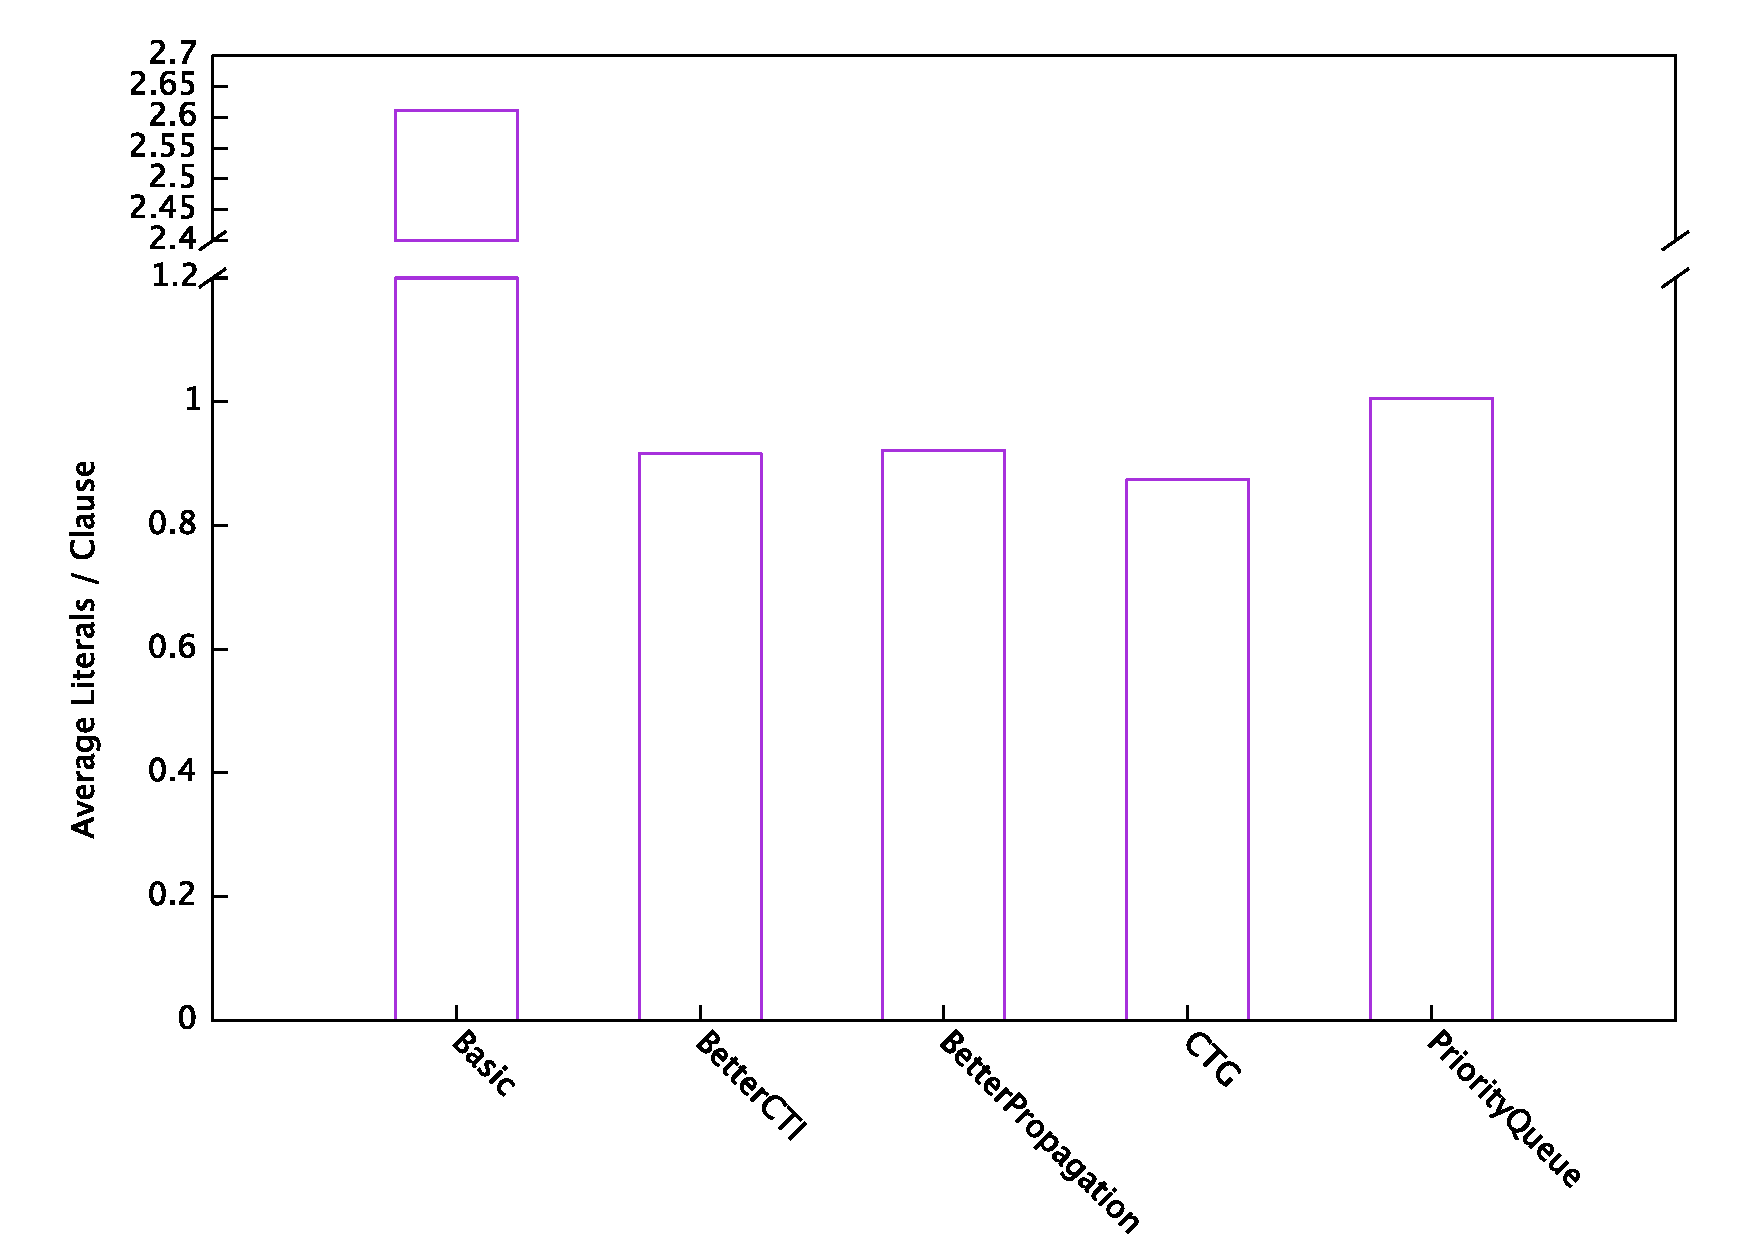
\includegraphics[width=16cm]{litspercls.pdf}
\caption{Average literals per clause averaged over the fourteen handwritten examples and fifty Hardware
Model Checking Competition examples.}
\end{figure}

\begin{figure}[!ht]
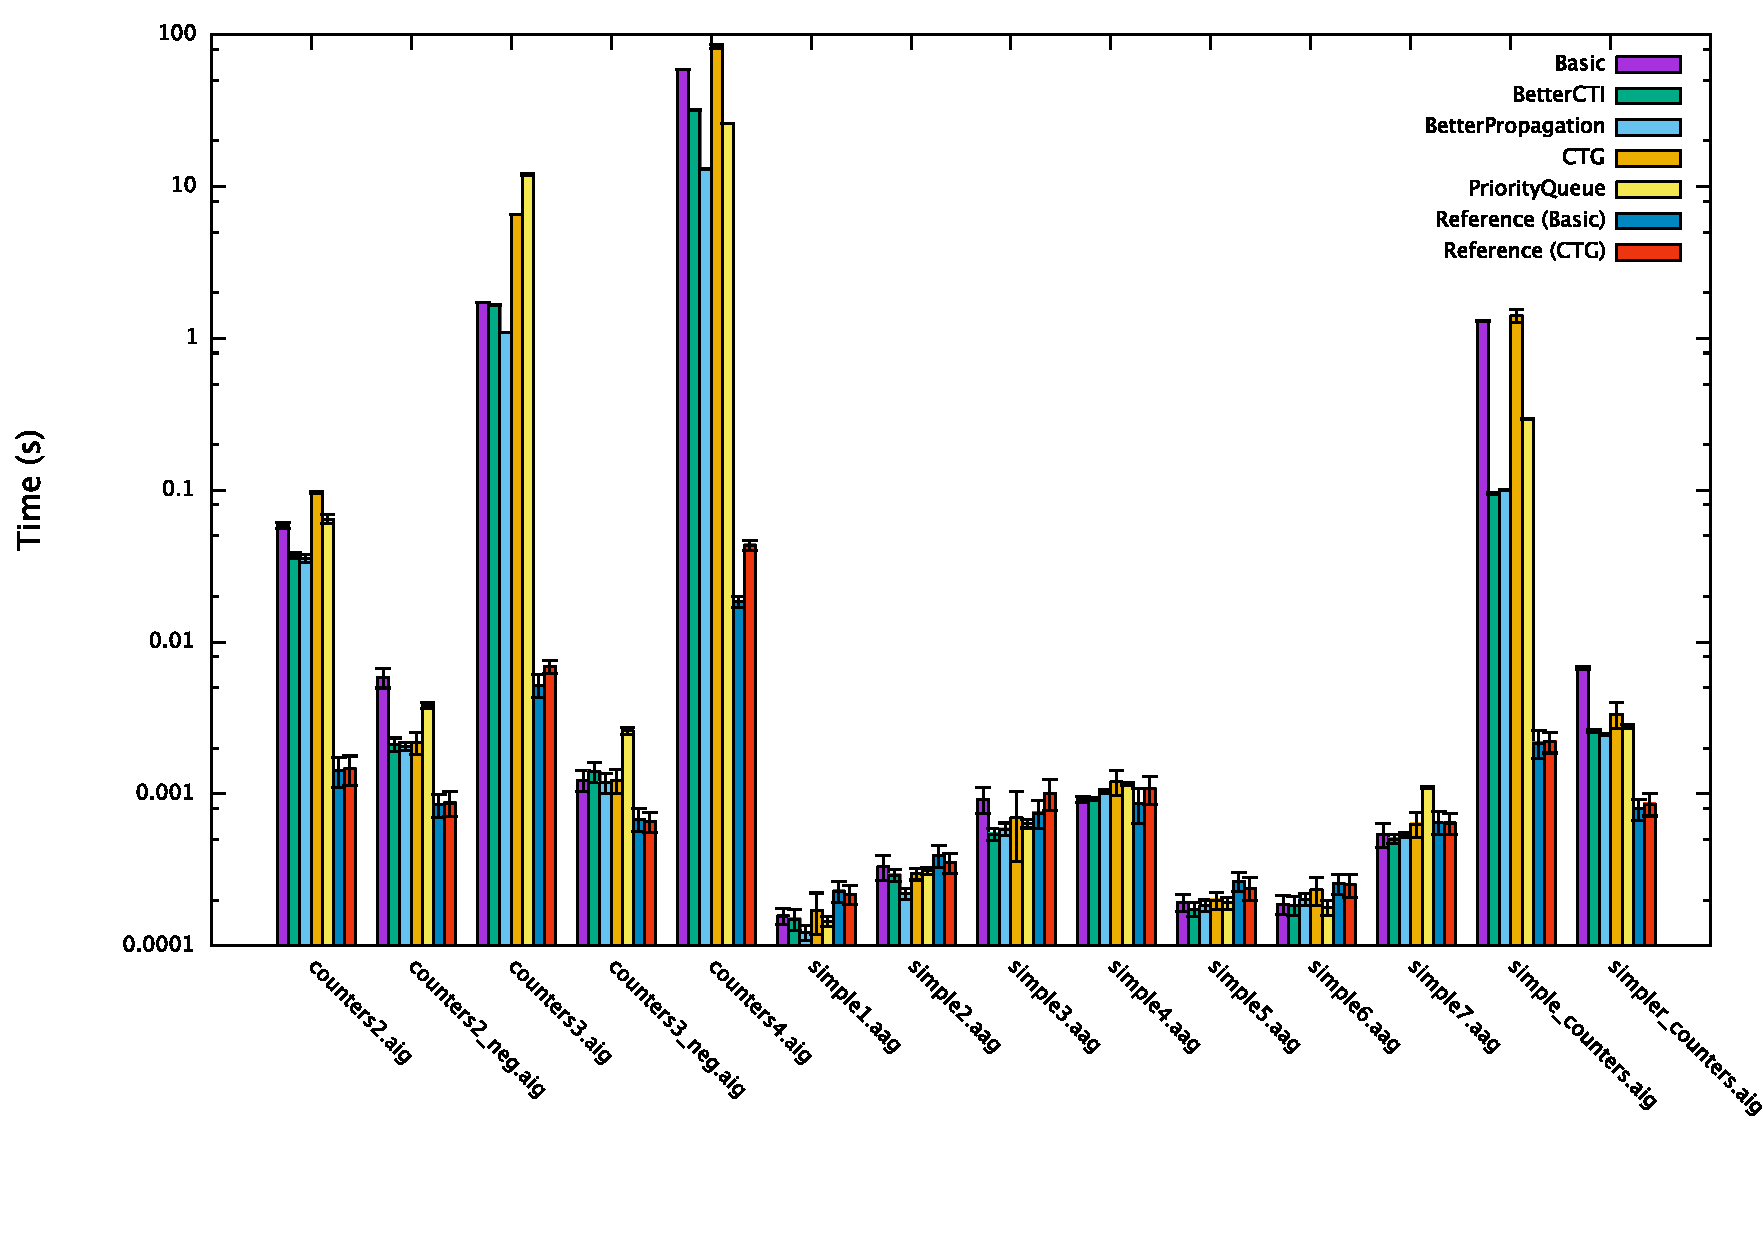
\includegraphics[width=16cm]{handwritten.pdf}
\caption{Benchmark results for the fourteen handwritten examples on a log scale.}
\end{figure}

\begin{figure}[!ht]
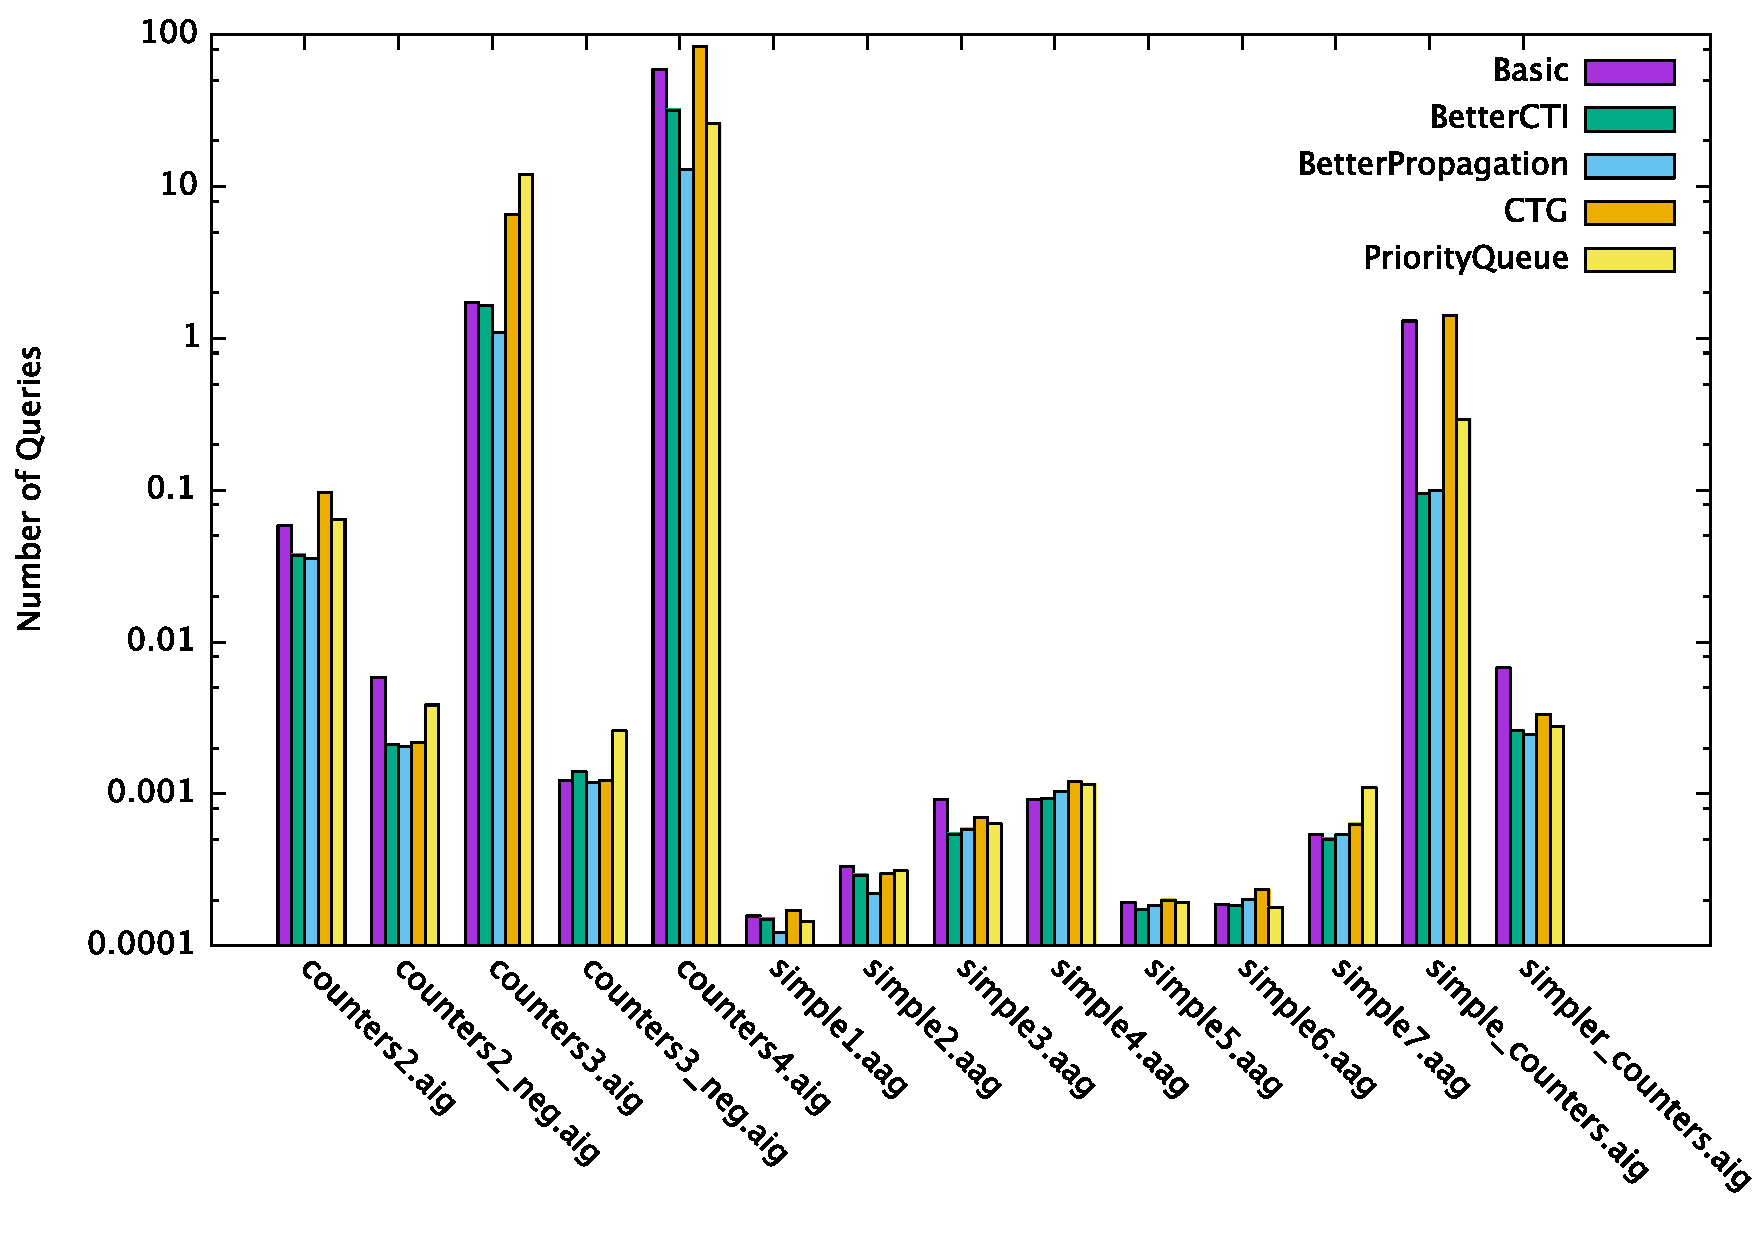
\includegraphics[width=16cm]{numqueries.pdf}
\caption{Number of queries for each variant run on the fourteen handwritten examples on a log scale.}
\end{figure}

\paragraph{Smaller Counterexamples to Induction}{
The \emph{BetterCTI} implementation exhibits consistently
better performance than the \emph{Basic} implementation for examples
that require finding at least one CTI. In such cases,
discovering CTI clauses with fewer literals leads, as expected, to a smaller average number of
literals per clause, which suggests smaller SAT queries.

As mentioned previously, because the \emph{BetterCTI} implementation uses
CTIs that encompass sets of states rather than single states, when a negated CTI is proven at a depth
$k$, several states have been shown to be unreachable within $k$ steps of the transition relation
from the initial state. Dealing with sets of states rather than single CTI states should allow
the \emph{BetterCTI} implementation to deal with fewer CTIs in some cases (because the CTI sets of states
may encompass several CTI states), leading to fewer queries needing to be made. Benchmark results
agree with these expectations; for examples that require finding more than one CTI, \emph{BetterCTI}
finds fewer CTIs and makes fewer queries. For example, the \emph{Basic} variant finds 59
CTIs and makes 414 queries to solve \verb,shortp0.aig,, but the \emph{BetterCTI} variant only
finds 3 CTIs and makes 49 queries.

The improvement of finding more general CTIs enabled the \emph{BetterCTI} variant of the implementation
(and all other implementations that include finding smaller CTIs) to
solve six more examples (\verb,counterp0.aig,, \verb,counterp0neg.aig,, \verb,pdtvishuffman7.aig,, 
\verb,pdtvismiim3.aig,, \verb,6s318r.aig,, \verb,srg5ptimo.aig,) than the \emph{Basic} version without
timing out.}

\paragraph{Propagation}{
Removing subsumed clauses also in results in better performance for several examples.
While the performance impact that the improvement has is less drastic than the improvement of
\emph{BetterCTI} over \emph{Basic} finding smaller CTIs, the \emph{BetterPropagation} version performs
considerably better
than the \emph{BetterCTI} version on the \verb,counters3.aig, and \verb,counters4.aig, examples in
particular, where the adjustments allow the algorithm to prove the safety properties using fewer
queries. Even for examples such as \verb,pdtvismiim3.aig,, where \emph{BetterPropagation} makes more
queries than \emph{BetterCTI}, \emph{BetterPropagation} manages to perform better than \emph{BetterCTI}
because it makes smaller queries.}

\paragraph{Counterexamples to Generalization}{
The \emph{CTG} variation that deals with CTGs performs worse than the \emph{BetterPropagation} version
on examples, even in cases where \emph{CTG} reduces the average number of frames per clause,
most likely because the examples used are too small for the performance benefits of using CTGs to
eliminate more states to overcome the overheads of finding and proving negated CTGs, which require
making additional queries on each call to the \verb,inductiveGeneralization, function.

Similar results can be found
in the performance of Aaron Bradley's reference implementation with basic generalization and
improved (CTG-using) generalization on the same examples: for these small examples,
the reference implementation performs better overall with CTG-handling disabled.}

\paragraph{Priority Queues}{
The \emph{PriorityQueue} implementation's performance generally does not perform as well as the
implementations that do not use priority queues (with the exception of \emph{CTG}). There are
two features of the variant in particular that may account for its worse performance: accumulating
CTIs and early generalization.

One of the performance advantages of the \emph{PriorityQueue} implementation is that CTIs do not need
to be rediscovered \cite{een11}: after a proof obligation $(s,i)$ is enqueued, until the algorithm fails or finds a fixed point,
the queue will always contain a proof obligation $(s,j)$ for $j \geq i$. When the proof obligation $(s,i)$
fulfilled at a certain depth $i$, $(s,i + 1)$ is then enqueued, If $s$ is a CTI for proving a property
$p$ at depth $i + 2$ (i.e. proof obligation $(\neg p, i + 2)$), by the time \verb,proveObligations, removes
proof obligation $(\neg p, i + 2)$ from the priority queue, $(s, i+1)$ has already been fulfilled, so the
CTI $s$ would not, after its initial discovery, need to be discovered again.

%As with the handling of CTGs, avoiding the rediscovery of CTIs may result in worse performance for smaller
%examples. Proof obligations that do not need to be fulfilled in order to find the fixed point may
%have to be proven in the \emph{PriorityQueue} implementation: even if $s$ is not a CTI for proving $p$
%at depth $i + 2$, the proof obligation $(s, i+1)$ would still need to be fulfilled before the
%\verb,proveObligations, attempts to fulfill $(\neg p, i + 2)$.

The \emph{PriorityQueue} implementation performs inductive generalization for each CTI only once, though,
when that CTI's first proof obligation is first enqueued. Rediscovering CTIs would allow the CTIs to
be generalized relative to later frames as well, rather than only to the first frame relative to which
the negated CTI is inductive. Not generalizing CTIs relative to later frames may lead to
\emph{PriorityQueue} making larger queries and explain the variant's higher average number of
literals per clause.
}

\section{Reference Implementation}
%Discuss performance comparison of final implementation with
%IC3 reference implementation, taking into account differences between
%the implementations.

The performance of this project's model checker implementations is, for all except very small examples
(e.g. \verb,simple1.aag,),
worse compared to the average performance of Aaron Bradley's reference implementation
(with or without generalization involving CTGs enabled).

The choice of implementation language may account for much of the difference in performance, as the reference
implementation in C++ has more control over memory allocations than the implementations in Haskell, which is
a garbage-collected language. I mention other differences between the implementations that may explain
some of the performance differences below.

\subsubsection{Model Representation}
The reference implementation differs from this project's implementations in representing the hardware model,
which may account for some of the performance differences.

The reference implementation keeps track of which variables are inputs, latches, and AND gates.
Each \verb,Model, maintains both the the primed and current values for inputs and latches and keeps a
table to memoize the values of AND gates.

%The next-state value for an unprimed variable is provided by a call to the \verb,primeVar, function in the
%\verb,Model, class, which returns the stored value for the corresponding primed variable
%if the variable is an input or latch. If the variable is the output of an AND gate, the \verb,Model,
%either returns a precomputed, stored value for that primed variable or calculates the value of the output
%of the AND gate, inserts the value into the AND table, and returns that value.

As mentioned earlier, when the consecution query $F_k \wedge T \Rightarrow P'$ fails, this corresponds
to the CNF query $F_k \wedge T \wedge \neg P'$ being satisfiable, and while a full satisfying assignment
$s$ gives a CTI state, it is better to use a set of states $c \subset s$ as a CTI cube, so that several
CTI states can be eliminated at once.
The \verb,stateOf, function uses the information kept in \verb,Model,s to extract the smaller
cube from the model $s$ giving the satisfying assignment for a failed consecution query directly,
without further SAT-solver queries.
The Haskell implementations instead use several SAT-solver queries to extract the necessary literals
from $s$.

\subsubsection{MiniSat}
The reference implementation is more closely coupled to MiniSat's implementation. Because both the reference
implementation and MiniSat are in C++, the reference implementation can and does call MiniSat functions
and instantiate MiniSat objects, such as \verb,SimpSolver,s directly. In contrast, the Haskell implementation
must interact with MiniSat through an interface and suffers from associated overheads, such as those from
marshalling data from the data structures returned from the C wrapper for MiniSat into the corresponding
Haskell data structures.

The reference implementation also makes use of empirical results to improve the performance of MiniSat queries.
For example, in the \verb,stateOf, function, which extracts a model from a failed consecution query
(to e.g. find a CTI cube), the set of literals passed to the MiniSat \verb,Solver, are reordered according
to an ordering of that was found to be the best choice empirically.

\subsubsection{Overall Structure}

The reference implementation uses a priority queue, but handles proof obligations differently
than the {\it PriorityQueue} implementation does. For a CTI $s$ that prevents the fulfillment
of a proof obligation at depth $i$, the reference implementation enqueues proof obligation $(s,i - 1)$
and performs generalization relative to the frame $F_{i - 1}$ each time $\neg s$ has been shown
to be inductive relative to frame $F_{i - 1}$ (generalization does not seem
to be as expensive for the reference implementation).
The reference implementation also does not
enqueue a new proof obligation $(s, i+1)$ each time a proof obligation $(s, i)$ has been
fulfilled as the {\it priorityQueue} implementation does, so CTIs need to be rediscovered.
The safety property is maintained and
handled separately from CTIs; its negation is not included as part of a proof obligation
placed in the priority queue.

\chapter{Conclusion}

This chapter summarizes the work done and goals met for this project. Following the summary, I give
suggestions for further extensions to the project.

\section{Summary}

The project aims to implement a basic version of the IC3 algorithm in Haskell with the necessary parser
and SAT-solver interface have been achieved, and the goal of the model checker being able to check
small example hardware model has also been reached. The \emph{Basic} implementation correctly
solved fourteen small examples, with its solutions agreeing with the solutions given by the
reference implementation of IC3.

In addition to the basic version of the IC3 algorithm, I implemented several variants of the model checker.
Furthermore the implementations of the model checker can model check not only
the fourteen handwritten hardware model examples but also models from the
Hardware Model Checking Competitions with thousands of variables.

I evaluated the different model checker variants by comparing their performance on examples from
the Hardware Model Checking Competition. The benchmark results show that finding smaller CTI clauses
results in a dramatic improvement in performance, with the best-performing implementation
\emph{betterPropagation} finding smaller CTI clauses and removing subsumed clauses from frames,
though none of the variants performs as well as the reference implementation of IC3.

\section{Further extensions}
Rather than implement the extensions mentioned in the initial project proposal, I elected to implement
other variants of the model checker and examine their effects on the model checker's performance.
As a result, interfacing with different SAT solvers remains a further extension. Additionally,
implementing further variants of the model checker remains as an extension.

Implementing interfaces with different SAT solvers may allow more examples to be solved efficiently.
Aaron Bradley notes that the performance of the IC3 algorithm is considerably affected
by the behavior of the SAT solver it uses \cite{bradley12}; even if each SAT query takes the same amount of
time, the algorithm's performance may still vary if the SAT solver behaves even slightly differently.
Because the choice of SAT solver may affect which examples can be solved efficiently, allowing the model
checker to use different SAT solvers may increase the number of examples that can be solved.

Other than using a different SAT solver, the performance of the model checker may be improved by
altering its overall structure. The current implementations of the model checker maintain one
\verb,Solver, per frame. A variant of the model checker that uses a single \verb,Solver,
instance may yield performance improvments, as suggested in several papers \cite{}.


%%%%%%%%%%%%%%%%%%%%%%%%%%%%%%%%%%%%%%%%%%%%%%%%%%%%%%%%%%%%%%%%%%%%%
% the bibliography
\addcontentsline{toc}{chapter}{Bibliography}
\bibliography{refs}

%%%%%%%%%%%%%%%%%%%%%%%%%%%%%%%%%%%%%%%%%%%%%%%%%%%%%%%%%%%%%%%%%%%%%
% the appendices
\appendix

\chapter{Benchmark Results}
\label{benchmarks}

\section{Basic}
\csvreader[longtable=|l|p{3em}|p{3.5em}|l|l|p{4.5em}|p{4em}|,
    table head= \hline Name & Frames & Avg. Lits / Clause & CTIs & Queries & Mean Time (s) & Std. Dev. of Time (s)\\\hline,
    late after line=\\\hline]%
{basic.csv}{name = \name, frames = \frames, litspercls = \litspercls, ctis = \ctis, queries = \queries, time = \time, stdev = \stdev}%
{\name & \frames & \litspercls & \ctis & \queries & \time & \stdev}%

\section{BetterCTI}
\csvreader[longtable=|l|p{3em}|p{3.5em}|l|l|p{4.5em}|p{4em}|,
    table head= \hline Name & Frames & Avg. Lits / Clause & CTIs & Queries & Mean Time (s) & Std. Dev. of Time (s)\\\hline,
    late after line=\\\hline]%
{betterCTI.csv}{name = \name, frames = \frames, litspercls = \litspercls, ctis = \ctis, queries = \queries, time = \time, stdev = \stdev}%
{\name & \frames & \litspercls & \ctis & \queries & \time & \stdev}%

\section{BetterPropagation}
\csvreader[longtable=|l|p{3em}|p{3.5em}|l|l|p{4.5em}|p{4em}|,
    table head= \hline Name & Frames & Avg. Lits / Clause & CTIs & Queries & Mean Time (s) & Std. Dev. of Time (s)\\\hline,
    late after line=\\\hline]%
{betterPropagation.csv}{name = \name, frames = \frames, litspercls = \litspercls, ctis = \ctis, queries = \queries, time = \time, stdev = \stdev}%
{\name & \frames & \litspercls & \ctis & \queries & \time & \stdev}%

\section{PriorityQueue}
\csvreader[longtable=|l|p{3em}|p{3.5em}|l|l|p{4.5em}|p{4em}|,
    table head= \hline Name & Frames & Avg. Lits / Clause & CTIs & Queries & Mean Time (s) & Std. Dev. of Time (s)\\\hline,
    late after line=\\\hline]%
{priorityQueue.csv}{name = \name, frames = \frames, litspercls = \litspercls, ctis = \ctis, queries = \queries, time = \time, stdev = \stdev}%
{\name & \frames & \litspercls & \ctis & \queries & \time & \stdev}%

\section{CTG}
\csvreader[longtable=|l|p{3em}|p{3.5em}|l|l|l|p{4.5em}|p{4em}|,
    table head= \hline Name & Frames & Avg. Lits / Clause & CTIs & CTGs & Queries & Mean Time (s) & Std. Dev. of Time (s)\\\hline,
    late after line=\\\hline]%
{ctg.csv}{name = \name, frames = \frames, litspercls = \litspercls, ctis = \ctis, ctgs = \ctgs, queries = \queries, time = \time, stdev = \stdev}%
{\name & \frames & \litspercls & \ctis & \ctgs & \queries & \time & \stdev}%

%\section{Reference Implementation}

\chapter{Project Proposal}

% A project proposal.
% The format draws heavily on the example project proposal
% and the Model Project Proposals (and their LaTeX sources) available
% http://www.cl.cam.ac.uk/teaching/projects/

\documentclass[12pt,a4paper,twoside]{article}
\usepackage[pdfborder={0 0 0}]{hyperref}
\usepackage[margin=25mm]{geometry}
\usepackage{graphicx}
\begin{document}

\section*{Introduction and Description of the Work}
Model checking is one way of assessing whether or not a hardware or
software system has certain properties. For example, model checkers can be
used to check systems for safety properties by finding examples of states
that violate the properties or by proving that all states have the
properties.

Explicit-state model checking can be infeasible for systems with a large
number of states, but symbolic model checking, which represents
states and the transition relation between them as boolean expressions,
can handle more states. Symbolic model checking initially relied on the
efficient representation of boolean expressions through binary decision
diagrams (BDDs), but BDDs can still consume a large amount of space, and
finding an ordering for BDD variables that keeps the BDDs small can become
costly \cite{biere99}.

Symbolic model checking techniques that rely on SAT solvers provide an
alternative to BDD-based approaches. SAT-based approaches include
bounded model checking \cite{biere99} and $k$-induction \cite{demoura03},
but both of these approaches involve unrolling the transition relation,
which can lead to long SAT solver queries.

IC3 \cite{bradley11} is a more recently developed SAT-based algorithm for
the symbolic model checking of safety properties. Instead of unrolling the
transition relation and considering entire paths, IC3 maintains a set of
frames $F_0,...,F_k$, where each frame $F_i$ is an overapproximation of
the set of states reachable in at most $i$ steps, and considers at most one
step of the transition relation from a particular frame at a time.
As a result, IC3 can find inductive strengthenings that tend
to be smaller and more convenient than those found by BMC-based
techniques such as $k$-induction, which finds strengthenings that are the
negations of spurious counterexample paths \cite{demoura03}, and the SAT
queries that IC3 makes tend to be simpler \cite{bradley12}.

This project focuses on implementing a symbolic model checker for verifying
safety properties of hardware. The model checker will include a new
implementation of the IC3 algorithm in Haskell, which will make use of an
existing SAT solver.

\section*{Starting Point}

I begin the project with some experience programming in Haskell
from a summer internship and no experience with model checking or using
a SAT solver. I have informally acquired some knowledge about model checking
to formulate this project idea.

\section*{Substance and Structure of the Project}

The project aims to implement a hardware model checker that takes its
inputs in AIGER format and queries the MiniSat SAT solver.

\noindent The structure of the project can be broken down into the following
components:

\begin{enumerate}

\item {\bf Parsing AIGER format} The model checker takes its inputs in AIGER
format and will, as a result, require an AIGER parser. The AIGER format
is fairly simple and hand-coding a parser for it should be suitable.

\item {\bf Interfacing with MiniSat} The model checker
will be using the MiniSat SAT solver, so an API that allows the
model checker to query MiniSat will be required.

\item {\bf Implementing the IC3 algorithm} 
The main aspect of the project is the implementation of the IC3 algorithm.
The implementation will largely be based on the algorithm as described in
\cite{bradley11,bradley12}. 

\item {\bf Evaluating the model checker}
The model checker will be evaluated by measuring its performance on
checking examples. Though the project does not focus greatly on the
efficiency of the implementation, it may still be interesting to
see how the performance of this IC3 implementation in Haskell compares with
other implementations. As a result, benchmarks taken for the
model checker will be compared with further benchmarks taken for
Aaron Bradley's reference IC3 implementation, which is
implemented in C++.
Given that the reference implementation takes its inputs in AIGER format
and also uses MiniSat, the benchmarks should provide a means to compare
the IC3 implementations specifically.

\item {\bf Writing the dissertation}

\end{enumerate}

\subsection*{Possible Extensions}
If the aforementioned aspects of the project are completed, carrying out
the following extensions could be possible:
\begin{itemize}
\item Interfacing with other SAT solvers, and possibly performing additional
benchmarking; comparing the performance of the model checker when used with
different SAT solvers may be of interest since the performance
of IC3 implementations tend to vary considerably depending on the
characteristics of the underlying SAT solver.
\item Model checking properties of real hardware as a case study.
\item Implementing abstraction-refinement as described in \cite{vizel12}.
\end{itemize}


\section*{Success Criteria}

The project will be a success if the following have been completed:
\begin{itemize}
\item The AIGER parser has been implemented.
\item The MiniSat interface has been implemented.
\item The IC3 algorithm has been implemented.
\item The model checker should be able to solve some small examples.
\end{itemize}


\section*{Timetable: Workplan and Milestones}

\begin{enumerate}

\item {\bf 16 October 2015 -- 28 October 2015}

Preliminary reading. Get familiar with the AIGER format, MiniSat and
relevant Haskell libraries and tools for implementing the components
of the project.

\item {\bf 29 October 2015 -- 4 November 2015}

Write an AIGER format parser.
\\
Milestone: Parser completed. Relevant information from
AIGER files can be extracted.

\item {\bf 5 November 2015 -- 18 November 2015}

Implement a MiniSat interface.
\\
Milestone: MiniSat interface completed, enabling the model checker to use
MiniSat to solve SAT problems.

\item {\bf 19 November 2015}

Begin implementing the IC3 algorithm.

\item {\bf Michaelmas vacation}

Continue implementing the IC3 algorithm.

\item {\bf 14 January 2016 -- 27 January 2016}

Write progress report. Finish implementation of the IC3 algorithm.
\\
Milestones: Progress report completed.
Working implementation of the model checker completed.

\item {\bf 28 January 2016 -- 10 February 2016}

Measure and compare this IC3 implementation's performance and the reference
implementation's performance.
\\
Milestone: Evaluation completed.

\item {\bf 11 February 2016 -- 11 March 2016}

Write the main parts of the dissertation.
\\
Milestone:
Finished writing main parts of dissertation: introduction, preparation,
implementation and evaluation chapters.

\item {\bf Easter vacation}

If necessary, use this time for catching up.
Otherwise, work on extensions, starting with interfacing with other
SAT solvers.
Finish writing dissertation.
\\
Milestones: All implementation and evaluation completed.
Draft dissertation completed.

\item {\bf 21 April 2016 -- 4 May 2016}

Proofread and edit dissertation as necessary.
\\
Milestone: Dissertation ready for submission.

\item {\bf 5 May 2016 -- 13 May 2016}

Time left for catching up in case any delays have occurred in the
completion of any milestones.
\\
Milestone: Dissertation submitted.

\end{enumerate}

\section*{Resources Required}

For the project I will mostly make use of my laptop, which runs OS X 10.8.
I accept full responsibility for this machine and I have made contingency
plans to protect myself against hardware and/or software failure. 
If my main computer fails, I will use MCS computers.
I will use GitHub for backup and git for revision control.

\noindent I will also be using:
\begin{itemize}
\item AIGER utilities, available \url{http://fmv.jku.at/aiger/}
\item MiniSat, available \url{https://github.com/niklasso/minisat}
\item Models from the Hardware Model Checking Competition, such as those
available \url{http://fmv.jku.at/hwmcc10/}
\item Aaron Bradley's Reference IC3 implementation, available
\url{https://github.com/arbrad/IC3ref}
\end{itemize}
\end{document}


\end{document}

